\documentclass[12pt,a4paper,oneside,titlepage]{article}

\usepackage{hyperref}
\usepackage{graphicx}
\usepackage{pgfgantt}
\usepackage{lscape}
\usepackage{verbatim}
\usepackage{cleveref}

\usepackage[a4paper]{geometry}

\begin{document}
\title{GC02 Team 7 Project Report \\ MINAP Mobile Application}
\author{Amer Kamil Zainal Abidin, Ke Wei, Marco Corrales Estrada}
\maketitle

\tableofcontents
\newpage
\section{Background}
\subsection{MINAP/NICOR}
The Myocardial Ischaemia National Audit Project (MINAP) investigates the management of heart attacks. Participating hospitals and ambulance services are provided with a record of their quality of management. These records are then compared to national and international clinical standards. The National Institute of Cardiovascular Outcomes Research (NICOR) is a partnership of clinicians, IT experts, analysts, academics and managers. Its mission is to "provide information to improve heart disease patients' quality of care and outcomes". Using different audits, MINAP being one of them, NICOR aims to provide the NHS, government and regulatory bodies real world data to be used in patient care \footnote{\href{http://www.ucl.ac.uk/nicor/audits/minap/publicreports}{MINAP Reports}}\footnote{\href{http://www.ucl.ac.uk/nicor}{NICOR Website}}. 

\subsection{Web Application}
Participating hospitals are requested to enter all patients with suspected heart attack into MINAP's central database system. Data are collected by nurses and other clinical audit staff and entered in a dedicated web application. This web application collects all patient data, from demographics to diagnosis and release information. As it stands, the web application contains a 130 field dataset that is updated every two years (latest revision, June 2013); it is currently only available to the web browser Internet Explorer versions 9 or below. The data is then validated against a set of rules which include, but are not limited to, value range checks, date range checks, data type checks and encryption rules. Once completed, records are stored on MINAP's Domino server\footnote{IBM Domino is used for enterprise collaboration, and is used primarily for its Lotus Notes capabilities in this instance}.

\subsection{Client}
The project's primary point of contact is Lucia Gavalova, Project Manager for the MINAP project, who we will refer to as the 'client' throughout this document (unless stated otherwise). Sue Manuel, MINAP's web app developer has also been a key stakeholder throughout the course of this project.

\newpage
\section{Requirements}
\textit{The following requirements have been formulated from a series of client meetings and e-mail communication, available in brief in ~\cref{sec:client}.}

\subsection{Overview}
Patient data record creation is currently restricted to when the nurses and other clinical audit staff are sitting in front of a computer. This would often be quite some time after a patient has been identified as being eligible for being entered into the MINAP dataset. A reduced-function mobile solution of the current web app was proposed by our client as a means of starting a patient record in MINAP's data set, allowing for prospective data collection. Completion of the record is expected to be done later on using the web app (using a full sized keyboard and screen).

\subsection{Use Cases}
The system's use case we are concerned with for our app can be modelled by the following table. Although the user-facing view of the system is fairly simple, most of the application logic lies in the interdependency and validation checks of the values entered by the user. 

\begin{center}
\begin{tabular}{|l|}
	\hline
	A nurse or clinical audit staff wants to create a record\\ \hline
	She first needs to login to the server with her credentials\\ \hline
	She then selects an option to create a new record\\ \hline
	She then is brought to a page to enter in her initial diagnosis\\ \hline
	If she doesn't understand a field, she can click on a button for help\\ \hline
	She then enters the patient details into a data input field\\ \hline
	If the data entered is invalid, a pop-up will appear, \\prompting her for correction\\ \hline
	She can then navigate through each page using 'next' buttons, \\or through a navigation map\\ \hline
	Throughout this process, she will save the data to the server by \\clicking a save button\\ \hline
	Once complete, she logs out of the system\\ \hline
	\end{tabular}
\end{center}
\subsection{Functional Requirements}
\subsubsection{User Authentication and Security}
As with the web application, the user must login to the central server prior to using the mobile app for data input. For security purposes, the user authentication details should not be held on the device beyond the initial authentication phase (or instead, use tokens), and all sensitive data retrieved from the server and created on the device should be destroyed at the end of a user session.
\subsubsection{Data Collection}
In order to create a patient record, the app needs to provide the user with forms for data entry. Depending on the data fields, certain format restrictions are imposed, for example: date and time related fields are in the dd/mm/yy hh:mm format; combo boxes; and numeric only data fields. Data fields should be divided into sections (pages) based on the current web app structure for familiarity. Data entered in by the user should be stored locally for the duration of the session, and ideally sent to a server once validated\footnote{See Data Submission}.
\subsubsection{Data Validation}
Validation currently occurs on the web app automatically at the point of exiting a data input object, page, or on saving. All 130 fields within the dataset must pass at least one validation rule. Certain fields will then either trigger additional validation rules involving other fields, default values to other fields, and/or open new sections of data collection to be filled out. Our app should follow this behaviour (with a subset of data) to ensure data integrity.
\subsubsection{Data Submission}
Once all mandatory data is entered and all validations rules have been passed, the user will be able to store the local record to a SQLite database. Due to time constraints, the team was unable to test calls to a web service of our own design as agreed with the client (20/11/13 Meeting). However, the SQLite database should prove to be flexible if used in future implementations as it is self-contained and follows the dataset's specifications.
\subsubsection{Mobile Usability}
Since the app will be running on smart phones (our target platform), factors such as the screen size, touch navigation, and use of an on-screen keyboard have to be taken into account during the user interface design phase. Certain features in the current web app (e.g. navigation and data submission) are not intuitive and need to be rethought for mobile use, but should still retain the familiarity of the existing interface. 

\subsection{Architectural Requirements}
The core purpose of our mobile application is to provide proof of concept for a solution what would offer a starting point for record creation. To that end, we came to a mutual agreement with the client that the original dataset be reduced from 130 fields. In exchange for reducing the volume of data, certain architectural requirements were requested so as to create a framework for future work to build upon (e.g. porting the application to other platforms).
\subsubsection{Web Services}
Although we have reached an agreement that we will not actually need to touch the live Domino Server, there are certain functions that our application will have to implement to ensure future compatibility with MINAP's technology stack (IBM Lotus Notes on Domino Server 8.5.3). Processes such as how data will be retrieved from the server and authentication processes should be modelled into the system as stubs that can be easily implemented at a later stage in the development of the app. Further research into the topic of communication with the server from other services was also deemed useful, since the client was unable to give a clear answer as to how this could be done.

\newpage
\section{Target Mobile Platform}
\subsection{Client Preference}
\subsection{Preliminary Research}
\subsection{User Survey}
THIS SECTION IS TO BE REWRITTEN
\\ \\
Our client has been unsure about the preferred target platform of the audience of our mobile app. To help better inform this decision, we have designed a user device survey which the client has agreed to running over the period of a few months, with a suggested completion date within 3 weeks of rolling out. The primary purpose of pushing out this survey is to better inform decisions of what secondary platforms should be supported to increase mobile app uptake by hospital staff. Despite this, due to the short time-frame imposed on us by GC01, we have mutually agreed to target Android mobile phones as the primary platform. More details regarding the device survey can be found in the Appendix.
\\ \\
THIS SECTION IS TO BE REWRITTEN

\newpage
\section{User Interface}
\subsection{Preliminary UI Design}
As part of ensuring our understanding of the requirements were in line with the client's expectations, we sketched out a preliminary user interface (UI) and presented our ideas to our client. The order in which each page was presented is indicated by red arrows. A summary of the key points relating to UI during our conversation are included below.

\subsubsection{Initial User Interface Feedback}
Client response:
\begin{itemize}
	\item happy with proposal of similar design to web app
	\item request for an application tutorial for "non-techie" users
	\item navigation menu: a simplified version of the map could be used for mobile
	\item an 'auto-save' feature would be useful ("like Microsoft Word") in case of battery loss, device breakage, or more pressing matters to attend to (i.e. emergency)
\end{itemize}
\subsubsection{Commentary and Response}
We have accepted the feedback from the client as being in line with our initial requirements. However, the request for an auto-save feature in the app would violate the privacy requirements of having volatile local data. A way to mitigate this would be to save the record to a 'draft' database when auto-saving (i.e. "submitting" a record without performing validation-on-send), but is a low-priority feature at this point.
\subsubsection{UI Tweaking}
After taking these comments on board, we have more formally modelled the user's flow of use through the app, mapping each UI element to Java's graphical implementation classes. It is worth noting that the UI is still in its initial stages, pending further adaptation for mobile use.

\subsection{Android UI Design}
Following the decision of designing for the Android platform,  ... more details on the design process can be found on the team's HCI blog.  General process and final product shown here with rationale to major design decisions.

\newpage
\section{Software Design}
\subsection{Systems Design}
\subsection{Designing for Android}
\subsection{Data Model \& Validation}
In order to capture the functional requirements previously explained, three major steps were to be completed for the inner workings of the mobile application.

\begin{figure}[h!]
\centering
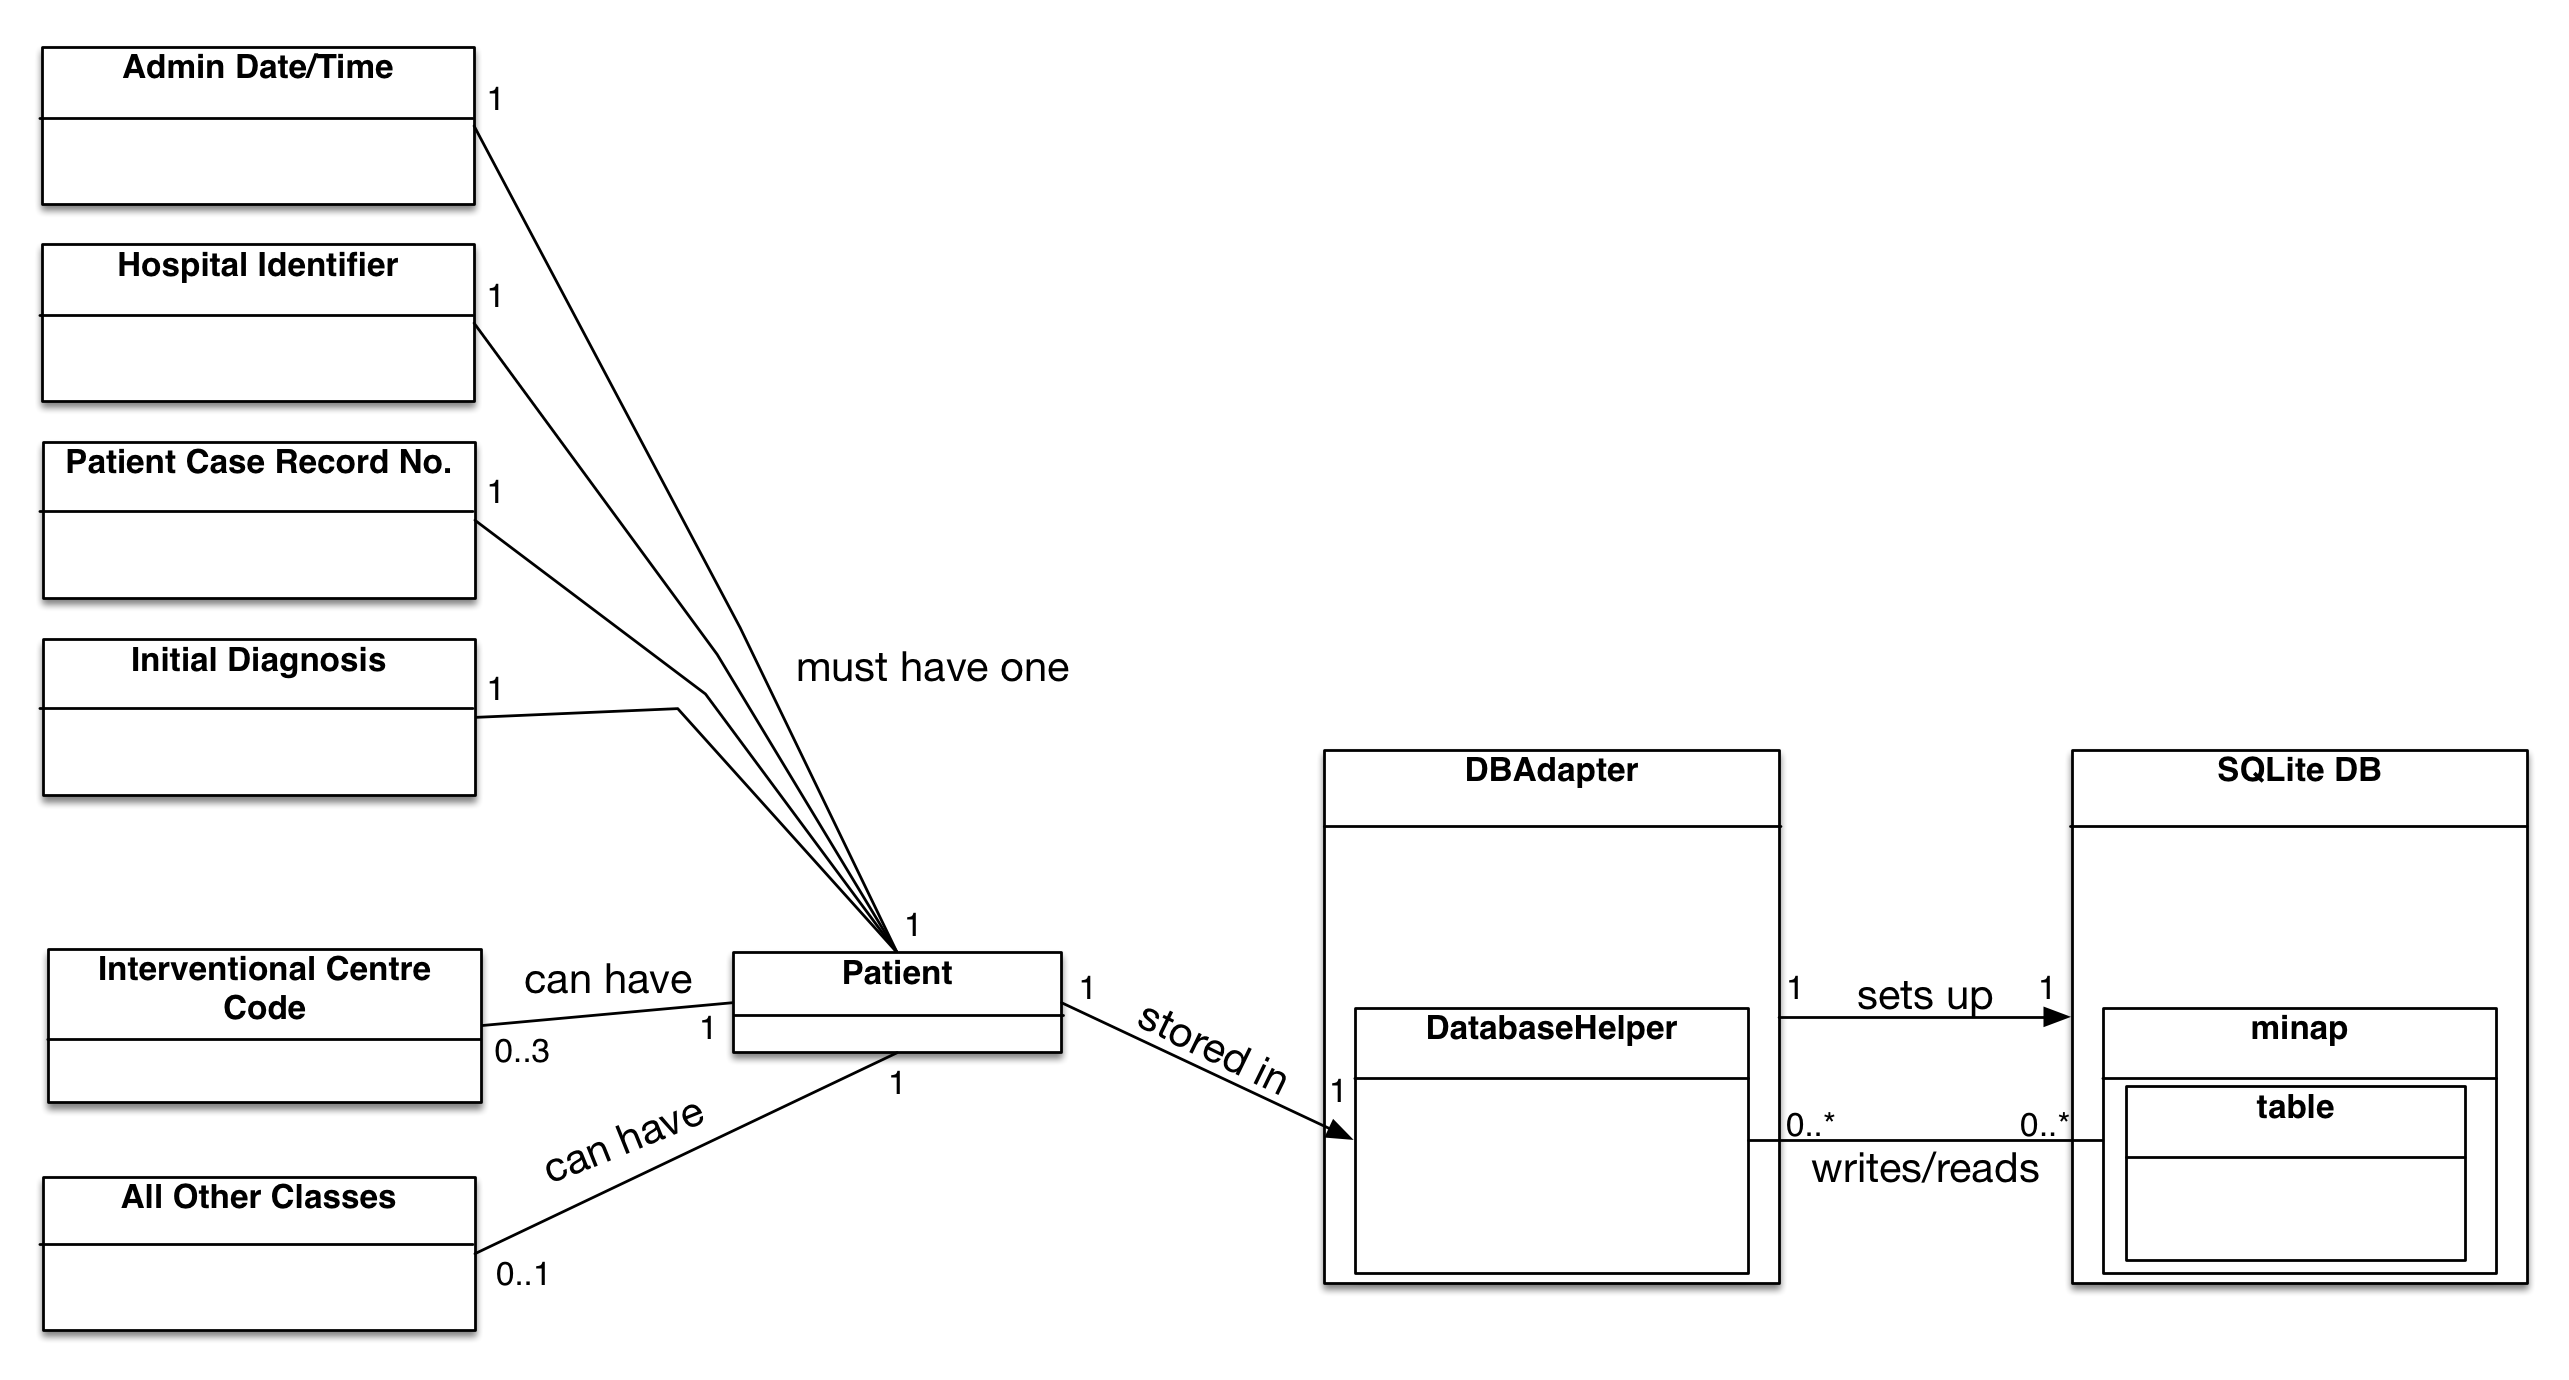
\includegraphics[scale=0.45]{img/database-class-diagram.png}
\caption{Database workflow class diagram}
\end{figure}

\subsubsection{Designing the patient singleton}
The Patient class would, in essence, capture the entirety of the dataset for this project. For security reasons, the team agreed with the client (5/12/13 Meeting) that the application should not hold more than one record per session. As such, the patient class was deemed fit to be designed as a Singleton. A call to a Patient object will return either an existent instance of the class or create one if such instance does not exist. Furthermore, the clone method of the Patient class has been overridden to throw a CloneNotSupported exception in order prevent stray clones from being created. All fields from the dataset are then declared as part of the patient class.

\subsubsection{Designing and implementing field classes and the Value superclass}
As previously mentioned, all fields must pass at least one validation rule before entering long term storage, either to the local database or MINAP's server. Although some fields shared similar validation rules, such as date fields needing a certain display format, the usage of a super class was minimized due to the volatility of the dataset itself. Due to this, our superclass, Value, only encapsulates variables that the team decided may not change as frequently as others; namely the field number within the dataset and the description of said field. These two values are used as tooltips on both the existing web application as well as our GUI. All field classes have been designed to be independent of each other.

Each class contains its own data validation rules. The MINAP dataset and sanity checks files provided by the client proved essential in deciding what data types to use for each field. Length check validations were handled by declaring a private short variable that would hold said length value. Date and time check validations were slightly trickier as they required the use of Date methods as well as importing the SimpleDateFormat library to better implement comparisons. Alphanumeric checks would need to be compared against regular expressions.

The getter methods would take an appropriate typed value as a parameter and return boolean true if said parameter passed the field's validation rules. An if statement was the most appropriate structure to check a parameter's value. Strings would need to clear regular expressions; Dates, Integers and Doubles have ranges they must fall within; to capture the drop down list or radio button behavior seen in the web application, classes with switch statements were implemented that both checked the selection for validity and set the fields "Long Code" variable to the appropriate value.

Setter methods, for reasons that will become clearer in the next session, would return the data necessary as a String in the needed display format.

\subsubsection{Designing and implementing the DB}
The SQLite database used in this project uses no third party libraries. It was clear that the less dependencies present in our code, the easier it may be to fully implement the dataset and network capabilities further down the road. As this approach was chosen, the implementation of the database was more time consuming than expected. The final result, however, was well worth it.

The database itself consists of only one table, one record long. The DBAdapter class starts by declaring the field names to be used, each logical "page" declaration finished by declaring an array of strings that can hold all column names to a particular page. The concatenateArrays method can then declare a larger array that will hold all columns that were previously declared, this method can and indeed is, then be used when a SELECT * statement needs to be used on the database. The database is then created by assigning it a name and a tag that will be used when updating the schema. After assigning the table a name, a String is declared that holds the SQL statement to create the database.

All of the database logic is held from the declaration of the DatabaseHelper class down. Methods to open and close the database are followed by methods that insert information to a set page, updating information in said pages. Special attention must be given to the insertPatient method as it represents the Patient Info page on the UI and is the only way to actually insert one more record onto the database. The DBAdapter class ends with the implementation of a method that will, due to the restriction of one record per session, destroy all data; and a method that will select all data from the record.

The columns on our patient table have all been set to be Text. This decision facilitates writing from the field classes getter methods without having to worry about server format compatibility. This decision, as well as the decision to only hold one record, can be easily expanded and corrected if necessary.

\newpage
\section{Testing \& Analytics}
\subsection{Automated Testing}

\subsection{Usage Analytics}
Although our mobile app is unlikely to be used by actual end-users in the near future, simple usage analytics were 

\newpage
\section{Application Limitations}
While this application does fulfil our client's requests, it is far from a finished product that could be implemented in the workplace. In order to provide a complete solution, our application would need to implement all missing fields from the dataset. These fields would then need to be reflected on the UI. However, the most obvious limitation of our solution is, without a doubt, the lack of network connectivity.

Our main priority during the second half of this project was to produce something tangible. To have something that our client could hold in her hands and, not to put it lightly, play with. To that end, and with her consent, networking research was put on the back burner in favour of delivering a functioning application.

Still, the need for a further study onto the networking technologies used at MINAP was necessary. If not for our project, for future hands to grapple with.

\subsection{Client-Server Communication}
As mentioned in the 20/11/13 Meeting, the team confirmed that making our app communicate with a Domino Server is not a key priority, and that spinning off another web server (e.g. Apache, + MSFT SQL Server) with a similar capabilities will satisfy the requirements. Therefore finding compatibility solutions between Java/Android and the Domino Server was reassigned as a research topic.

The aim of the research was to understand the domino web server communication protocol, to some degree, as it could help explore the possibility of making our app cross-platform and future-proof. With little understanding on the topic, I started with searching through the user guide for Domino 8.5 (IBM.COM) and found out that Domino supports Web services as defined in the W3C documents Simple Object Access Protocol (SOAP) 1.1 and Web Services Description Language (WSDL) 1.1.

SOAP (Simple Object Access Protocol) is a protocol specification for exchanging structured information in the implementation of Web Services within computer networks. It relies on the XML Information Set for its message format, and usually makes use of other Application Layer protocols, most notably Hypertext Transfer Protocol (HTTP) or Simple Mail Transfer Protocol (SMTP), for message negotiation and transmission.

The official SOAP Version 1.1 specification document has been added to resources used (W3.com). It provides not only background informations of SOAP, but also extensive knowledge how a SOAP message is constructed, how to use SOAP in HTTP, and examples of SOAP messages.

As an example of how SOAP procedures can be used, a SOAP message could be sent to a web service-enabled site; such as a real-estate price database, with the parameters needed for a search. The site would then return an XML-formatted document with the resulting data, e.g., prices, location, features. With the data being returned in a standardized machine-parsable format, it can then be integrated directly into a third-party web site or application.
\\ \\
A SOAP message is simply an XML file which contains the following elements:

\begin{itemize}
	\item An Envelope element that identifies the XML document as a SOAP message
	\item A Header element that contains header information
	\item A Body element that contains call and response information
	\item A Fault element containing errors and status information
\end{itemize}
A basic structure of a SOAP message is offered (w3schools.com): 

\begin{figure}[h!]
\centering
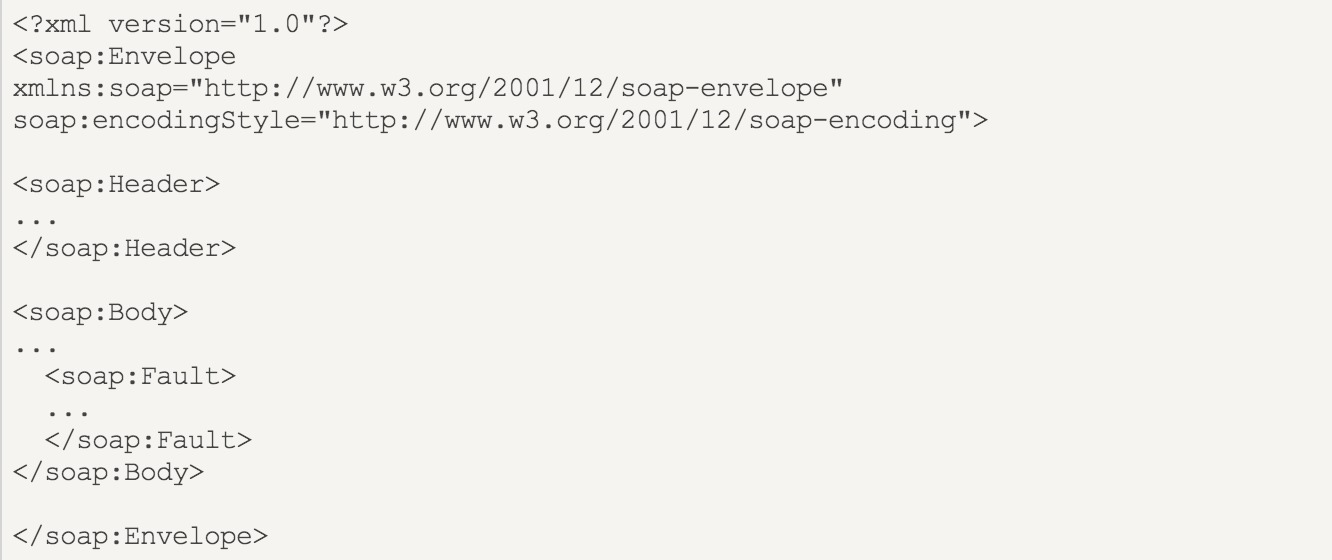
\includegraphics[scale=0.7]{img/soap-1.jpg}
\caption{Basic structure of a SOAP message \cite{soap1}}
\end{figure}

Examples of SOAP Messages (w3schools.com): In this example, a "GetStockPrice" was sent to the test server (\url{http://www.example.org/stock}). As a response, the "Price" value was returned.

\begin{figure}[h!]
\centering
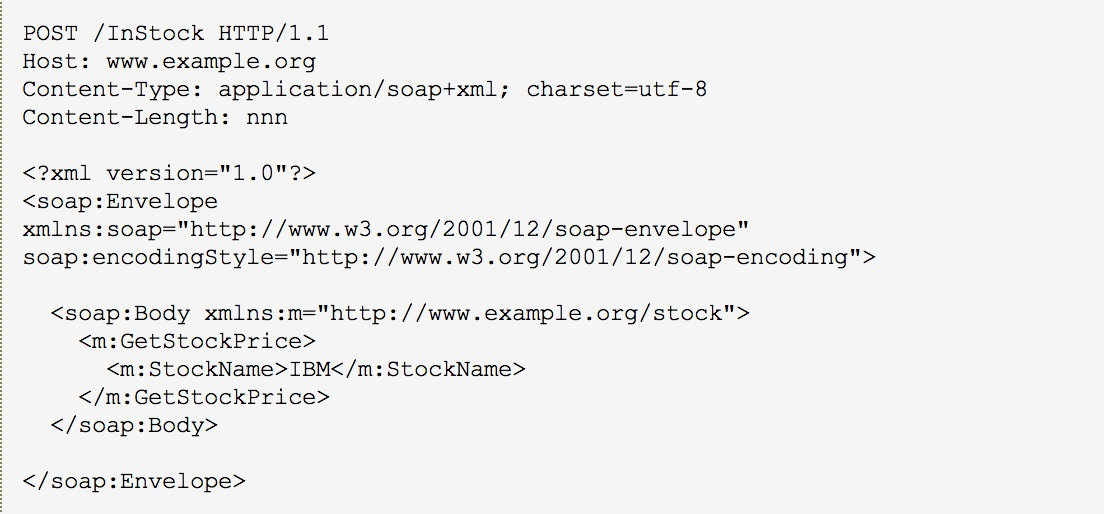
\includegraphics[scale=0.7]{img/soap-2.jpg}
\caption{Example HTTP Request}
\end{figure}

\begin{figure}[h!]
\centering
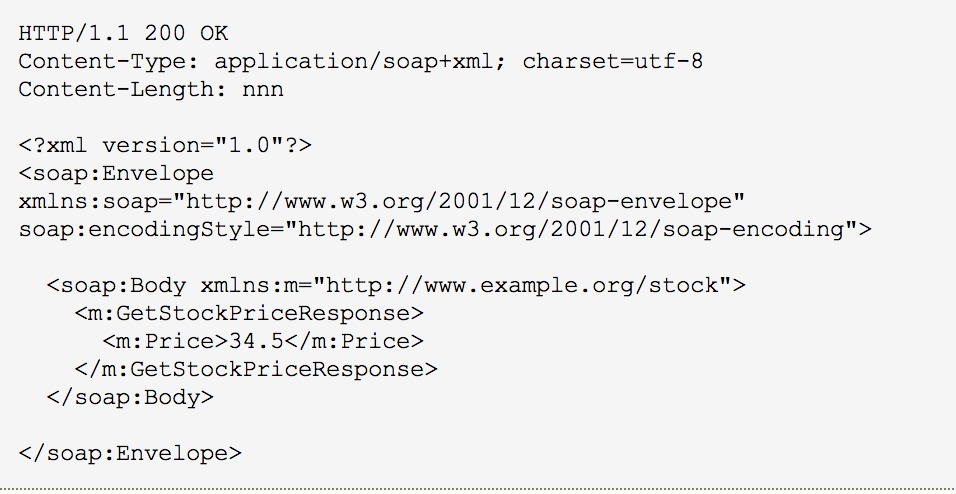
\includegraphics[scale=0.7]{img/soap-3.jpg}
\caption{Example HTTP Response}
\end{figure}

In terms of the real world implementation of the communication between Domino and Android device, many sources were found online, however few of them were actually helpful to this research. In the end, an interesting web page called How to Call Web Service in Android Using SOAP was found (c-sharpcorner.com). From what I have gathered so far, it seems Android does not provide any sort of SOAP library; according to the web page, our best bet is kSOAP 2. It is a SOAP web service client library for constrained Java environments such as Applets or J2ME applications (CLDC / CDC / MIDP). In the webpage that was mentioned before, a connection between an Android device and a non-Domino web service was established through SOAP. Since the Domino web server supports SOAP, with modifications it should be possible to establish a connection between an Android device and the Domino web server. In future research, this should be attempted.

\newpage
\section{Client Feedback}

\newpage
\section{Future Plans}
\subsection{Use of XML/Portable Data Files}
The application rules are currently defined by a series of data fields stored across two excel spreadsheets. From what we understand (20/11/13 Meeting), these rules are implemented in client-side Javascript for the current web app. Ideally, these rules would need to be stored in a standard machine-readable format which can be easily translated to validation code in any programming language.

\newpage
\section{Project Management}


\subsection{Work Packages}



\begin{landscape}
\subsection{Gantt Chart}
\begin{ganttchart}[
	hgrid,
	vgrid,
	time slot format=isodate
	]{2013-11-01}{2013-11-30}
	\gantttitlecalendar{year, month=name, day} \\
	\ganttgroup{Requirements Gathering}{2013-11-01}{2013-11-15} \\
	\ganttmilestone{GC01 Milestone 1}{2013-11-24} \ganttnewline
	\ganttgroup{InitialDevelopment}{2013-11-16}{2013-11-30} \\
\end{ganttchart}

\newpage

\begin{ganttchart}[
	hgrid,
	vgrid,
	time slot format=isodate
	]{2013-12-01}{2013-12-31}
	\gantttitlecalendar{year, month=name, day} \\
	\ganttmilestone{GC01 Milestone 2}{2013-12-20} \ganttnewline
\end{ganttchart}

\newpage

\begin{ganttchart}[
	hgrid,
	vgrid,
	time slot format=isodate
	]{2014-01-01}{2014-01-28}
	\gantttitlecalendar{year, month=name, day} \\
	\ganttmilestone{GC02 Final Milestone}{2014-01-27} 
\end{ganttchart}

\end{landscape}

\newpage
\section{Teamwork}
\subsection{Team Roles}
Team roles were initially assigned based on the recommended list provided in the GC01 document requirements. These team roles were useful as a set of guidelines leading up to the first project milestone, but we quickly found that the assignment of multiple formal roles to team members was unrealistic for such a fast-paced project with team members at various skill levels. This meant that roles previously assigned to team members were not always reflective of their current work package, as the rest of the team pitched in to complete critical unfinished packages. As such, only the roles which the team member was most active in are tabulated below:
\\ \\
\begin{table}[h]
\centering
    \begin{tabular}{ | p{5cm} | p{5.4cm} |}
    \hline
    Name & Active Roles \\ \hline
    Marco \textbf{David} Corrales \newline (Secondary Team Lead) & Secondary Developer \newline Data/Database Designer \newline \\ \hline
     Amer \textbf{Kamil} Zainal \newline (Primary Team Lead)  & Primary Developer \newline Systems Designer \& Analyst \newline Documentation Lead \newline \\ \hline
     \textbf{Ke} Wei & Networking Researcher \newline \\ \hline
    \end{tabular}
    \caption{Team Member Active Roles}
    \end{table}

\newpage
\subsection{Teamwork Commentary}
\subsubsection{Team Workflow}
\paragraph{Trello} ~\\
\href{https://trello.com}{Trello}\footnote{Information disclosed on Trello are private to the team} has been used extensively by the team for information organisation. Agendas for the next meeting are typically decided at the end of each meeting, with unfinished items of the day deferred; ensuring that each agenda is a summary of what was achieved at each meeting. To supplement this, any details (e.g. comments, photos, resources) related to the meeting are included in a separate section with a corresponding date. 
\begin{figure}[h!]
\centering
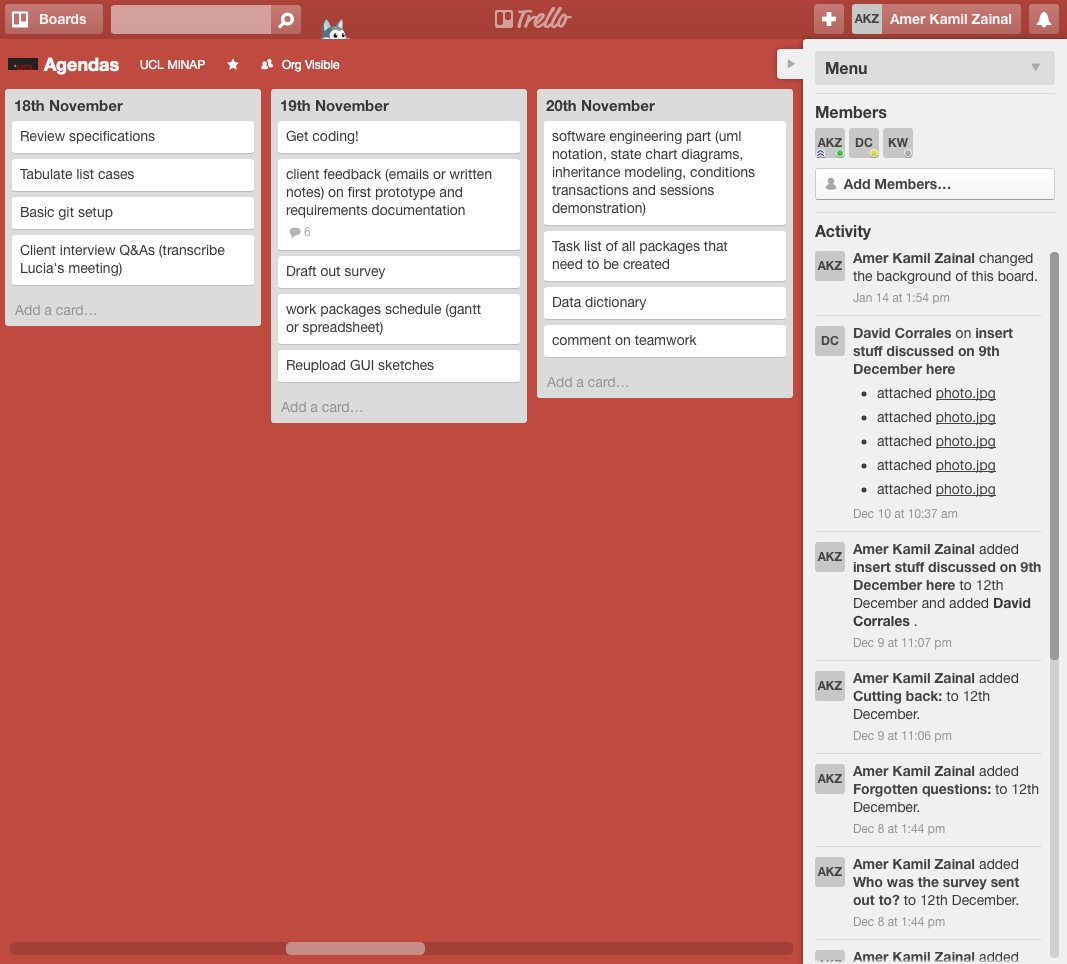
\includegraphics[scale=0.35]{img/trello.png}
\caption{Snapshot of a board in the team's Trello}
\end{figure}
\\
\newpage
\paragraph{GitHub} ~\\
To further consolidate our memory of team progress, David updated a \href{http://akz08.github.io/minap-mobile/}{blog} \\(http://akz08.github.io/minap-mobile/) on \href{http://pages.github.com/}{GitHub Pages} using \href{http://octopress.org/}{Octopress}, summarising our meeting outcomes up to our first academic milestone. Due to the public nature of blogs, we initially ensured to omit any client identifying information to avoid any potential privacy problems, however we later decided that this was unnecessarily restrictive. This openness of communication was also necessary for us to write about our design process for the HCI requirement of our blog. All of the blog posts created are tagged with the author's name for attribution.

For source code collaboration, we used a private \href{https://github.com}{GitHub} repository which was worked on by all members of the team. GitHub's repository wiki functionality was used for collaboration of more long-form documentation (e.g. writing this report) and structured ordering of resources. Due to the varying experience levels with git, the team mostly made use of simple git branches for each person. A full copy of the git repository is included in the project source code submission for closer inspection, contributing to the large file size. 

\begin{figure}[h!]
\centering
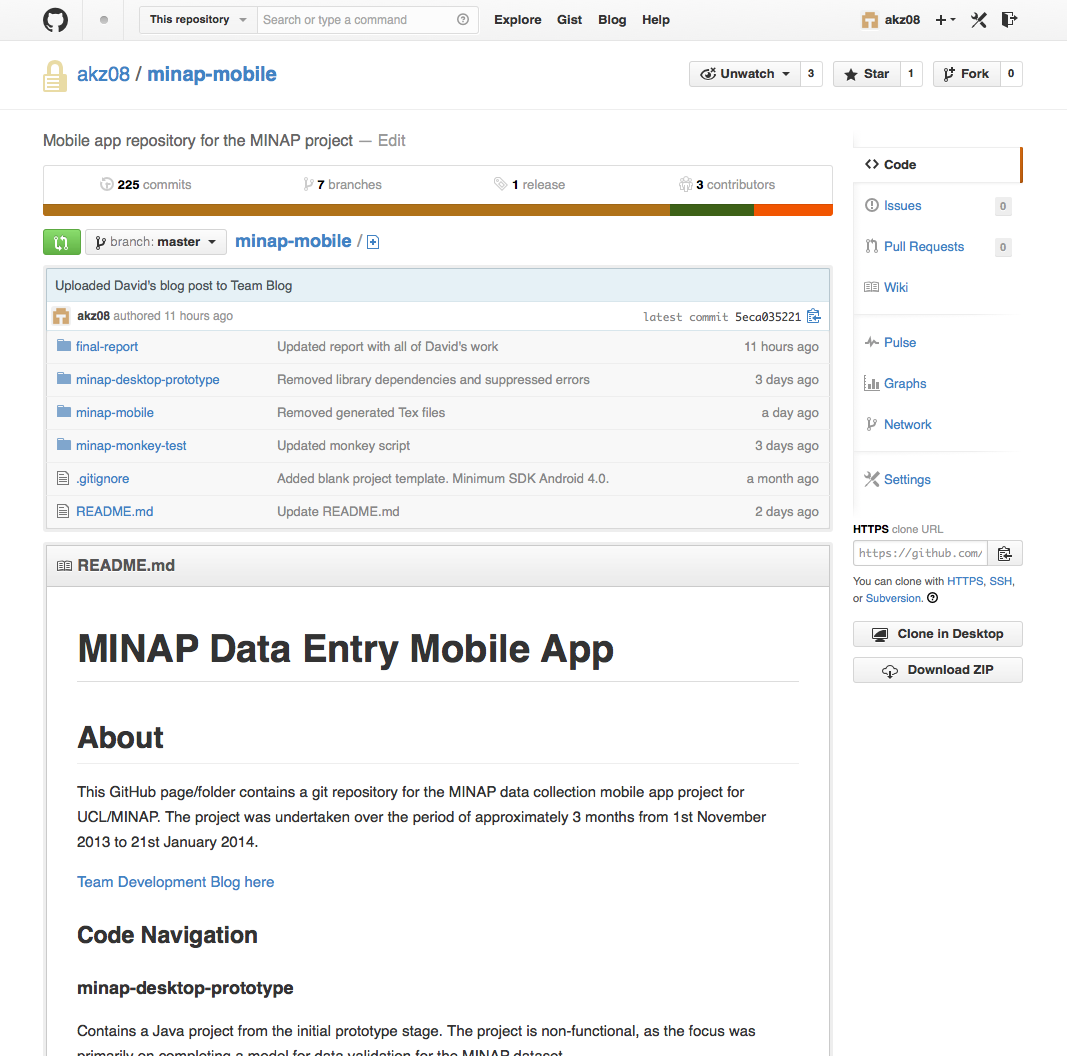
\includegraphics[scale=0.3]{img/github.png}
\caption{Snapshot of the team's GitHub repository page}
\end{figure}
\paragraph{Flowdock} ~\\
For a unified cross-platform communication service, and to avoid having to check both Trello and GitHub frequently, we also used \href{https://www.flowdock.com/}{FlowDock} extensively to easily track changes and keep each other updated. The service also allowed team members to control the level of notifications, to avoid a constant barrage of information (as well as work-life separation).

The service proved to be especially useful in tracking the progress of work packages, allowing other members to intervene if the pace of work was noticeably slower than expected. 
\begin{figure}[h!]
\centering
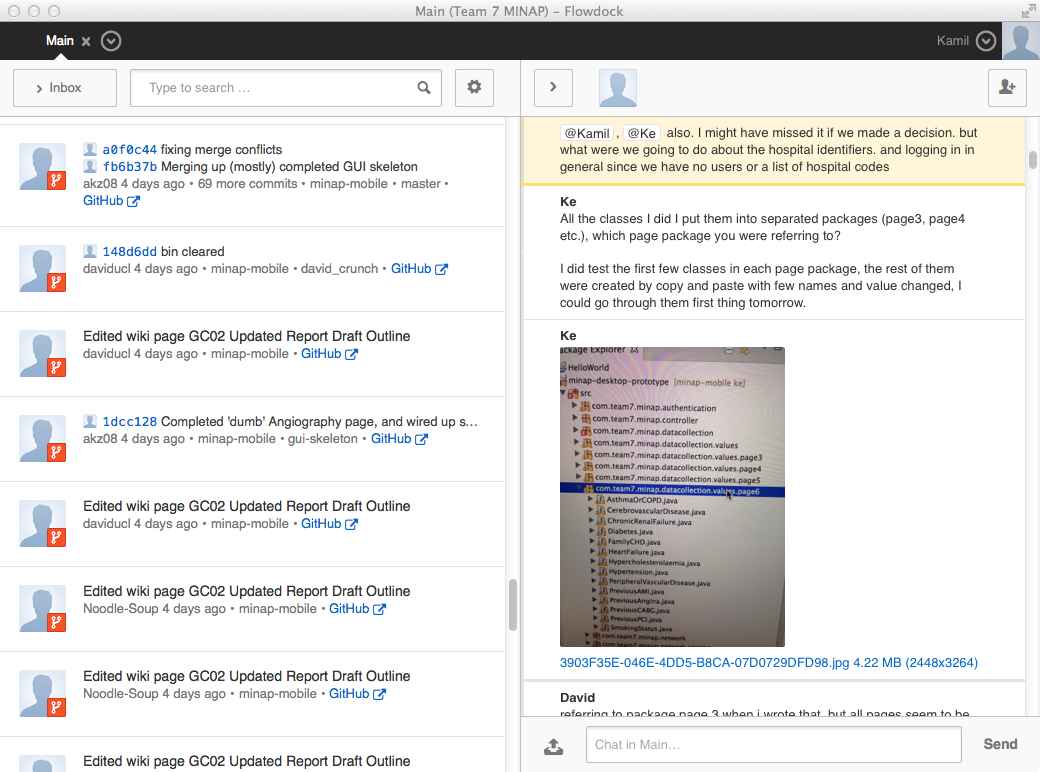
\includegraphics[scale=0.4]{img/flowdock.png}
\caption{Snapshot of the team's Flowdock activity}
\end{figure}
\subsubsection{Task Assignment}
Team members typically were assigned work packages by the team leader, based on their current capabilities. These tended to be general work outlines, and were negotiable in their scope. The decisions on work packages at any given time were strongly influenced by ongoing technology research, the current state of the overall system, and client feedback.
\subsubsection{Meetings}
The team typically met every workday to complete work together up to the first academic milestone. Most meetings since then have been conducted informally online using Flowdock, with occasional in-person catch-up meetings. This structure was more suited to the team once working on the final product, as work by each member was mostly independent of each other. Snapshots of early team meetings can be found in ~\cref{sec:internal_meetings}. 

\newpage
\begin{thebibliography}{9}

\bibitem{soap1}
w3schools.com, Example of SOAP message: \url{http://www.w3schools.com/webservices/ws_soap_syntax.asp}

\bibitem{domino}
ibm.com, Domino 8.5 user guide: \url{http://publib.boulder.ibm.com/infocenter/domhelp/v8r0/index.jsp?topic=%2Fcom.ibm.designer.domino.main.doc%2FH_EXAMPLES_WEB_SERVICES.html}

\bibitem{soap2}
w3.org, SOAP document from W3: \url{http://www.w3.org/TR/2000/NOTE-SOAP-20000508/}

\bibitem{ksoap}
kSOAP: \url{http://ksoap2.sourceforge.net/}

\bibitem{csharpc}
C\# Corner, How to Call Web Service in Android Using SOAP: \url{http://www.c-sharpcorner.com/UploadFile/88b6e5/how-to-call-web-service-in-android-using-soap/}

\end{thebibliography}

\newpage
\appendix
\newgeometry{left=1cm}
\section{Data Dictionary}
\subsection{Patient Class}

\begin{center}
	\begin{tabular}{| p{13cm} | p{5cm} |}
	\hline
	\textbf{AdminStatus} & \textbf{$<<$extends Value$>>$} \\ \hline
	\textasciitilde com.ucl.appteam7.minapmobile.model.values.DemographicsAdmission	 & \\ \hline
	$<<$import$>>$ com.ucl.appteam7.minapmobile.model.Value& \\ \hline \hline
	- \underline{adminStatus} : Byte & Holds the short code for patient's admission status \\ \hline
	- \underline{statusLongCode} : String & Holds the long code associated with adminStatus  \\ \hline \hline
	+ $<<$constructor$>>$ AdminStatus() & Sets the appropriate superclass values \\ \hline	
	+ \underline{setAdminStatus}(admStatus : Byte) : Boolean & Returns true if parameter passes validation rules \\ \hline	
	+ \underline{getAdminStatus}() : String & Returns the selected short code and corresponding long code as a String \\ \hline	
	+ \underline{getLongCode}() : String & Returns the long code associated with adminStatus variable \\ \hline	
	\end{tabular}
\end{center}

\begin{center}
	\begin{tabular}{| p{13cm} | p{5cm} |}
	\hline
	\textbf{AdmissionAfterNSTEMI} & \textbf{$<<$extends Value$>>$} \\ \hline
	\textasciitilde com.ucl.appteam7.minapmobile.model.values.InitialDiagnosis & \\ \hline
	$<<$import$>>$ com.ucl.appteam7.minapmobile.model.Value & \\ \hline \hline
	- \underline{admissionAfterSTEMI} : Boolean = false & Holds a boolean value, reveals items on UI \\ \hline \hline
	+ $<<$constructor$>>$ AdmissionAfterNSTEMI() & Sets the appropriate superclass values \\ \hline
	+ \underline{setAdmissionAfterSTEMI}(admASTEMI : Boolean) : Boolean & Sets, then returns admissionAfterSTEMI \\ \hline
	+ \underline{getAdmissionAfterSTEMI}() : String & Returns a String value of admissionAfterSTEMI \\ \hline
	\end{tabular}
\end{center}

\begin{center}
	\begin{tabular}{| p{13cm} | p{5cm} |}
	\hline
	\textbf{AdmissionDate} & \textbf{$<<$extends Value$>>$} \\ \hline
	\textasciitilde com.ucl.appteam7.minapmobile.model.values.PatientInfo & \\ \hline
	$<<$import:$>>$ com.ucl.appteam7.minapmobile.model.Value; & \\ \hline
	$<<$import:$>>$ java.text.ParseException; & \\ \hline
	$<<$import:$>>$ java.text.SimpleDateFormat; & \\ \hline
	$<<$import:$>>$ java.util.Date; & \\ \hline \hline
	- \underline{adminDate} : String & Holds Date String, formatted as needed \\ \hline
	- \underline{adminTime} : String & Holds Time String, formatted as needed \\ \hline
	- \underline{adminDateTime} : String & Combines both previous variables \\ \hline
	- \underline{now} : Date = new Date() & Holds the current date, used for validation \\ \hline
	\underline{sd} : SimpleDateFormat = new SimpleDateFormat("dd/mm/yyyy") & Holds the String format desired for adminDate \\ \hline
	\underline{st} : SimpleDateFormat = new SimpleDateFormat("HH:mm") & Holds the String format desired for adminTime \\ \hline
	\underline{sdt} : SimpleDateFormat = new SimpleDateFormat("dd/mm/yyy HH:mm") & Holds the String format for adminDateTime \\ \hline \hline
	+ $<<$constructor$>>$ AdmissionDate() & Sets the appropriate superclass values \\ \hline
	+ \underline{setDateTime}() : Boolean & Checks date and time validation, returns true if passed \\ \hline
	+ \underline{setADate}(aDate : Date) : Boolean & Checks the passed Date against date validation rules, returns true if passed \\ \hline
	+ \underline{setATime}(aTime : Date) : Boolean & Checks the passed Date against time validation rules, returns true if passed \\ \hline
	+ \underline{getDateTime}() : String & Returns adminDateTime variable \\ \hline
	+ \underline{getADate}() : String & Returns adminDate variable \\ \hline
	+ \underline{getATime}() : String & Returns adminTime variable \\ \hline
	\end{tabular}
\end{center}

\begin{center}
	\begin{tabular}{| p{13cm} | p{5cm} |}
	\hline
	\textbf{AdmissionMethod} & \textbf{$<<$extends Value$>>$} \\ \hline
	\textasciitilde com.ucl.appteam7.minapmobile.model.values.DemographicsAdmission & \\ \hline
	$<<$import$>>$ com.ucl.appteam7.minapmobile.model.Value & \\ \hline \hline
	- \underline{admissionMethod} : Byte & Holds the short code for patient's admission method \\ \hline
	- \underline{admissionLongCode} : String & Holds the long code associated with admissionMethod \\ \hline \hline
	+ $<<$constructor$>>$ AdmissionMethod() & Sets the appropriate superclass values \\ \hline
	+ \underline{setAdmissionMethod}(admMethod : Byte) : Boolean & Returns true if parameter passes validation rules \\ \hline
	+ \underline{getAdmissionMethod}() : String & Returns the selected short code and corresponding long code as a String \\ \hline
	+ \underline{getLongCode}() : String & Returns the long code associated with admissionMethod variable \\ \hline
	\end{tabular}
\end{center}

\begin{center}
	\begin{tabular}{| p{13cm} | p{5cm} |}
	\hline
	\textbf{AdmissionWard} & \textbf{$<<$extends Value$>>$} \\ \hline
	\textasciitilde com.ucl.appteam7.minapmobile.model.values.DemographicsAdmission & \\ \hline
	$<<$import$>>$ com.ucl.appteam7.minapmobile.model.Value & \\ \hline \hline
	- \underline{admissionWard} : Byte & Holds the short code for patient's admission ward \\ \hline
	- \underline{wardLongCode} : String & Holds the long code associated with admissionWard \\ \hline \hline
	+ $<<$constructor$>>$ AdmissionWard() & Sets the appropriate superclass values \\ \hline
	+ \underline{setAdmissionWard}(admWard : Byte) : Boolean & Returns true if parameter passes validation rules \\ \hline
	+ \underline{getAdmissionWard}() : String & Returns the selected short code and corresponding long code as a String \\ \hline
	+ \underline{getLongCode}() : String & Returns the long code associated with admissionWard variable \\ \hline
	\end{tabular}
\end{center}

\begin{center}
	\begin{tabular}{| p{13cm} | p{5cm} |}
	\hline
	\textbf{AdmittingConsultant} & \textbf{$<<$extends Value$>>$} \\ \hline
	\textasciitilde com.ucl.appteam7.minapmobile.model.values.DemographicsAdmission & \\ \hline
	$<<$import$>>$ com.ucl.appteam7.minapmobile.model.Value & \\ \hline \hline
	- \underline{admittingConsultant} : Byte & Holds the short code for patient's admitting consultant
 \\ \hline
	 - \underline{consulLongCode} : String & Holds the long code associated with admittingConsultant \\ \hline \hline
	 + $<<$constructor$>>$ AdmittingConsultant() & Sets the appropriate superclass values \\ \hline
	 + \underline{setAdmittingConsultant}(admConsul : Byte) : Boolean & Returns true if parameter passes validation rules \\ \hline
	 + \underline{getAdmittingConsultant}() : String & Returns the selected short code and corresponding long code as a String \\ \hline
	 + \underline{getLongCode}() : String & Returns the long code associated with admittingConsultant variable \\ \hline
	\end{tabular}
\end{center}

\begin{center}
	\begin{tabular}{| p{13cm} | p{5cm} |}
	\hline
	\textbf{AngioDate} & \textbf{$<<$extends Value$>>$} \\ \hline
	\textasciitilde com.ucl.appteam7.minapmobile.model.values.Angiography & \\ \hline
	$<<$import$>>$ com.ucl.appteam7.minapmobile.model.Value & \\ \hline
	$<<$import$>>$ java.text.ParseException & \\ \hline
	$<<$import$>>$ java.text.SimpleDateFormat & \\ \hline
	$<<$import$>>$ java.util.Date & \\ \hline \hline
	\underline{sd} : SimpleDateFormat = new SimpleDateFormat("dd/mm/yyyy") & Holds the String format desired for angioDate \\ \hline
	\underline{st} : SimpleDateFormat = new SimpleDateFormat("HH:mm") & Holds the String format desired for angioTime \\ \hline
	\underline{sdt} : SimpleDateFormat = new SimpleDateFormat("dd/mm/yyyy HH:mm") & Holds the String format desired for angioDateTime \\ \hline
	- \underline{angioDate} : String & Holds the patient's angiography date \\ \hline
	- \underline{angioTime} : String & Holds the patient's angiography time \\ \hline
	- \underline{angioDateTime} : String & Holds the patient's angiography date and time \\ \hline
	- \underline{$DATE\_FORMAT$} : String = "01/01/2000" & Lower bound for date range check \\ \hline
	- \underline{now} : Date = new Date() & Holds current Date, used for range check \\ \hline \hline
	+ $<<$constructor$>>$ AngioDate() & Set the appropriate superclass values \\ \hline
	+ \underline{setDateTime}() : Boolean & Returns true if both dates passed validation \\ \hline
	+ \underline{setangioralDate}(rDate : Date) : Boolean & Returns true if Date parameter passes validation \\ \hline
	+ \underline{setangioralTime}(rTime : Date) : Boolean & Returns true if Time parameter passes validation \\ \hline
	+ \underline{getDateTime}() : String & Returns angioDateTime variable \\ \hline
	+ \underline{getAngioDate}() : String & Returns angioDate variable \\&\\ \hline
	+ \underline{getAngioTime}() : String & Returns angioTime variable \\ &\\ \hline
	\end{tabular}
\end{center}

\begin{center}
	\begin{tabular}{| p{13cm} | p{5cm} |}
	\hline
	\textbf{AngioDelay} & \textbf{$<<$extends Value$>>$} \\ \hline
	\textasciitilde com.ucl.appteam7.minapmobile.model.values.Angiography & \\ \hline
	$<<$import$>>$ com.ucl.appteam7.minapmobile.model.Value & \\ \hline \hline
	- \underline{angioDelay} : Byte & Holds the short code for patient's angiography delay \\ \hline
	- \underline{angioDelayLongCode} : String & Holds the long code associated with angioDelay \\ \hline \hline
	+ $<<$constructor$>>$ AngioDelay() & Sets the appropriate superclass values \\ \hline
	+ \underline{setAngioDelay}(aDelay : Byte) : Boolean & Returns true if parameter passes validation rules \\ \hline
	+ \underline{getAngioDelay}() : String & Returns the selected short code and corresponding long code as a String \\ \hline
	+ \underline{getLongCode}() : String & Returns the long code associated with angioDelay variable \\ \hline
	\end{tabular}
\end{center}

\begin{center}
	\begin{tabular}{| p{13cm} | p{5cm} |}
	\hline
	\textbf{AsthmaOrCOPD} & \textbf{$<<$extends Value$>>$} \\ \hline
	\textasciitilde com.ucl.appteam7.minapmobile.model.values.MedicalHistory & \\ \hline
	$<<$import$>>$ com.ucl.appteam7.minapmobile.model.Value & \\ \hline \hline
	- \underline{asthmaCOPD} : Byte & Holds the short code for patient's cerebrovascular disease status \\ \hline
	- \underline{asthmaCOPDLongCode} : String & Holds the long code associated with asthmaCOPD \\ \hline \hline
	+ $<<$constructor$>>$ AsthmaOrCOPD() & Sets the appropriate superclass values \\ \hline
	+ \underline{setAsthmaCOPD}(cDisease : Byte) : Boolean & Returns true if parameter passes validation rules \\ \hline
	+ \underline{getAsthmaCOPD}() : String & Returns the selected short code and corresponding long code as a String \\ \hline
	+ \underline{getLongCode}() : String & Returns the long code associated with asthmaCOPD variable \\ \hline
	\end{tabular}
\end{center}

\begin{center}
	\begin{tabular}{| p{13cm} | p{5cm} |}
	\hline
	\textbf{BMI} & \textbf{$<<$extends Value$>>$} \\ \hline
	\textasciitilde com.ucl.appteam7.minapmobile.model.values.Examinations & \\ \hline
	$<<$import$>>$ com.ucl.appteam7.minapmobile.model.Value & \\ \hline \hline
	- \underline{bmi} : Double & Holds the patient's BMI \\ \hline \hline
	+ $<<$constructor$>>$ BMI() & Set the appropriate superclass values \\ \hline
	+ \underline{setBMI}(height : Double, weight : Double) : Boolean & Calculates BMI, returns true if parameter passes validation \\ \hline
	+ \underline{getBMI}() : String & Returns bmi as a formatted String \\ \hline
	\end{tabular}
\end{center}

\begin{center}
	\begin{tabular}{| p{13cm} | p{5cm} |}
	\hline
	\textbf{CerebrovascularDisease} & \textbf{$<<$extends Value$>>$} \\ \hline
	\textasciitilde com.ucl.appteam7.minapmobile.model.values.MedicalHistory & \\ \hline
	$<<$import$>>$ com.ucl.appteam7.minapmobile.model.Value & \\ \hline
	- \underline{cerebrovascularDisease} : Byte & Holds the short code for patient's cerebrovascular disease status \\ \hline
	- \underline{cerebrovascularDiseaseLongCode} : String & Holds the long code associated with cerebrovascularDisease \\ \hline \hline
	+ $<<$constructor$>>$ CerebrovascularDisease() & Sets the appropriate superclass values \\ \hline
	+ \underline{setCerebrovascular}(cDisease : Byte) : Boolean & Returns true if parameter passes validation rules \\ \hline
	+ \underline{getCerebrovascular}() : String & Returns the selected short code and corresponding long code as a String \\ \hline
	+ \underline{getLongCode}() : String & Returns the long code associated with cerebrovascularDisease variable \\ \hline
	\end{tabular}
\end{center}

\begin{center}
	\begin{tabular}{| p{13cm} | p{5cm} |}
	\hline
	\textbf{ChronicRenalFailure} & \textbf{$<<$extends Value$>>$} \\ \hline
	\textasciitilde com.ucl.appteam7.minapmobile.model.values.MedicalHistory & \\ \hline
	$<<$import$>>$ com.ucl.appteam7.minapmobile.model.Value & \\ \hline \hline
	- \underline{chronicRenalFailure} : Byte & Holds the short code for patient's chronic renal failure status \\ \hline
	- \underline{chronicRenalFailureLongCode} : String & Holds the long code associated with chronicRenalFailure \\ \hline \hline
	+ $<<$constructor$>>$ ChronicRenalFailure() & Sets the appropriate superclass values \\ \hline
	+ \underline{setRenalFailure}(cRenalFailure : Byte) : Boolean & Returns true if parameter passes validation rules \\ \hline
	+ \underline{getRenalFailure}() : String & Returns the selected short code and corresponding long code as a String \\ \hline
	+ \underline{getLongCode}() : String & Returns the long code associated with chronicRenalFailure variable \\ \hline
	\end{tabular}
\end{center}

\begin{center}
	\begin{tabular}{| p{13cm} | p{5cm} |}
	\hline
	\textbf{CoronaryAngiography} & \textbf{$<<$extends Value$>>$} \\ \hline
	\textasciitilde com.ucl.appteam7.minapmobile.model.values.Angiography & \\ \hline
	$<<$import$>>$ com.ucl.appteam7.minapmobile.model.Value & \\ \hline \hline
	- \underline{coronaryAngiography} : Byte & Holds the short code for patient's coronary angiography \\ \hline
	- \underline{coronaryAngiographyLongCode} : String & Holds the long code associated with coronaryAngiography \\ \hline \hline
	+ $<<$constructor$>>$ CoronaryAngiography() & Sets the appropriate superclass values \\ \hline
	+ \underline{setCoronaryAngiography}(cAngiography : Byte) : Boolean & Returns true if parameter passes validation rules \\ \hline
	+ \underline{getCoronaryAngiography}() : String & Returns the selected short code and corresponding long code as a String \\ \hline
	+ \underline{getLongCode}() : String & Returns the long code associated with coronaryAngiography variable \\ \hline
	\end{tabular}
\end{center}

\begin{center}
	\begin{tabular}{| p{13cm} | p{5cm} |}
	\hline
	\textbf{CoronaryIntervention} & \textbf{$<<$extends Value$>>$} \\ \hline
	\textasciitilde com.ucl.appteam7.minapmobile.model.values.Angiography & \\ \hline
	$<<$import$>>$ com.ucl.appteam7.minapmobile.model.Value & \\ \hline \hline
	- \underline{coronaryIntervention} : Byte & Holds the short code for patient's coronary intervention \\ \hline
	- \underline{coronaryInterventionLongCode} : String & Holds the long code associated with coronaryIntervention \\ \hline \hline
	+ $<<$constructor$>>$ CoronaryIntervention() & Sets the appropriate superclass values \\ \hline
	+ \underline{setCoronaryIntervention}(cIntervention : Byte) : Boolean & Returns true if parameter passes validation rules \\ \hline
	+ \underline{getCoronaryIntervention}() : String & Returns the selected short code and corresponding long code as a String \\ \hline
	+ \underline{getLongCode}() : String & Returns the long code associated with coronaryIntervention variable \\ \hline
	\end{tabular}
\end{center}

\begin{center}
	\begin{tabular}{| p{13cm} | p{5cm} |}
	\hline
	\textbf{DaycaseTransferDate} & \textbf{$<<$extends Value$>>$} \\ \hline
	\textasciitilde com.ucl.appteam7.minapmobile.model.values.Angiography & \\ \hline
	$<<$import$>>$ com.ucl.appteam7.minapmobile.model.Value & \\ \hline
	$<<$import$>>$ java.text.ParseException & \\ \hline
	$<<$import$>>$ java.text.SimpleDateFormat & \\ \hline
	$<<$import$>>$ java.util.Date & \\ \hline \hline
	\underline{sd} : SimpleDateFormat = new SimpleDateFormat("dd/mm/yyyy") & Holds the String format desired for daycaseDate \\ \hline
	- \underline{daycaseDate} : String & Holds the patient's daycase transfer date \\ \hline
	- \underline{$DATE\_FORMAT$} : String = "01/01/2000" & Lower bound for date range check \\ \hline
	- \underline{now} : String = sd.format(new Date()) & Holds current Date as a String, used for range check \\ \hline \hline
	+ $<<$constructor$>>$ DaycaseTransferDate() & Set the appropriate superclass values \\ \hline
	+ \underline{setDaycaseDate}(iDate: Date) : Boolean & Returns true if parameter passes validation \\ \hline
	+ \underline{getDaycaseDate}() : String & Returns daycaseDate variable \\ \hline
	\end{tabular}
\end{center}

\begin{center}
	\begin{tabular}{| p{13cm} | p{5cm} |}
	\hline
	\textbf{DBAdapter} & \textbf{Holds all SQLite logic} \\ \hline
	\textasciitilde com.ucl.appteam7.minapmobile.model & \\ \hline
	$<<$import$>>$ java.util.Collections & \\ \hline
	$<<$import$>>$ java.util.Date & \\ \hline
	$<<$import$>>$ java.util.List & \\ \hline
	$<<$import$>>$ java.util.ArrayList & \\ \hline
	$<<$import$>>$ android.content.ContentValues & \\ \hline
	$<<$import$>>$ android.content.Context & \\ \hline
	$<<$import$>>$ android.database.Cursor & \\ \hline
	$<<$import$>>$ android.database.SQLException & \\ \hline
	$<<$import$>>$ android.database.sqlite.SQLiteOpenHelper & \\ \hline
	$<<$import$>>$ android.database.sqlite.SQLiteDatabase & \\ \hline
	$<<$import$>>$ android.util.Log & \\ \hline \hline
	+ \underline{$HOSPITAL\_IDENTIFIER$} : String = "HospitalID" & Declares HospitalID as a column for a database's table \\ \hline
	+ \underline{$RECORD\_NO$} : String = "RecordNum" & Declares RecordNum \\ \hline
	+ \underline{$NHS\_NUMBER$} : String = "NHSNumber" & Declares NHSNumber \\ \hline
	+ \underline{$PATIENT\_SURNAME$} : String = "PatientSurname" & Declares PatientSurname \\ \hline
	+ \underline{$PATIENT\_FORENAME$} : String = "PatientForename" & Declares PatientForename \\ \hline
	+ \underline{$PATIENT\_DOB$} : String = "PatientDOB" & Declares PatientDOB \\ \hline
	+ \underline{$ADMISSION\_DATE$} : String = "AdminDate" & Declares AdminDate \\ \hline
	+ \underline{$PATIENT\_INFO$} : String[] = \{$HOSPITAL\_IDENTIFIER, RECORD\_NO, $ $NHS\_NUMBER, PATIENT\_SURNAME,$ $PATIENT\_FORENAME, PATIENT\_DOB, $ $ADMISSION\_DATE$\} & Compiles previous columns for the Patient Info page \\ \hline 
	+ \underline{$INITIAL\_DIAGNOSIS$} : String = "InitialDiagosis" & Declares InitialDiagnosis \\ \hline
	+ \underline{$ADMISSION\_AFTER\_NSTEMI$} : String = "AdminStemi" & Declares AdminStemi \\ \hline
	+ \underline{$HIGH\_RISK\_NSTEMI$} : String = "HiRisknSTEMI" & Declares HiRisknSTEMI \\ \hline
	+ \underline{$INTERVENTIONAL\_PROCEDURE$} : String = "InterventionalProcedure" & Declares InterventionalProcedure \\ \hline
	+ \underline{$RETURN\_TO\_REFERRING\_HOSPITAL$} : String = "ReferHospitalReturn" & Declares ReferHospiralReturn \\ \hline
	+ \underline{$INTERVENTIONAL\_CENTRE\_CODE\_ID$} : String = "InterventionCentreCode" & Declares InterventionCentreCode \\ \hline
	\end{tabular}
\end{center}	
	
\begin{center}
	\begin{tabular}{| p{13cm} | p{5cm} |}
	\hline
	+ \underline{$DIAGNOSIS$} : String[] =  \{$INITIAL\_DIAGNOSIS, $ $ADMISSION\_AFTER\_NSTEMI, $ $HIGH\_RISK\_NSTEMI, $ $INTERVENTIONAL\_PROCEDURE, $& Compiles previous columns for Initial Diagnosis page\\  $RETURN\_TO\_REFERRING\_HOSPITAL, $ &\\ $INTERVENTIONAL\_CENTRE\_CODE\_ID$\} &  \\ \hline
	+ \underline{$PATIENT\_GENDER$} : String = "Gender" & Declares Gender \\ \hline
	+ \underline{$PATIENT\_ETHNICITY$} : String = "Ethnicity" & Declares Ethnicity \\ \hline
	+ \underline{$ADMISSION\_METHOD$} : String = "AdminMethod" & Declares AdminMethod \\ \hline
	+ \underline{$ADMISSION\_WARD$} : String = "AdminWard" & Declares AdminWard \\ \hline
	+ \underline{$GP\_PCT\_CODE$} : String = "GPCode" & Declares GPCode \\ \hline
	+ \underline{$PATIENT\_POST\_CODE$} : String = "PostCode" & Declares PostCode \\ \hline
	+ \underline{$ADMITTING\_CONSULTANT$} : String = "AdminConsul" & Declares AdminConsul \\ \hline
	+ \underline{$ADMISSION\_STATUS$} : String = "AdminStatus" & Declares AdminStatus \\ \hline
	+ \underline{$PLACE\_FIRST\_12\_LEAD\_ECG\_PERFORMED$} : String = "FirstECG" & Declares FirstECG \\ \hline
	+ \underline{$NHS\_VERIFICATION$} : String = "NHSVerif" & Declares NHSVerif \\ \hline
	+ \underline{$REFERRAL\_HOSPITAL$} : String = "RefHospital" & Declares RefHospital \\ \hline
	+ \underline{$ADMISSION$} : String[] = \{$PATIENT\_GENDER, $ $PATIENT\_ETHNICITY, ADMISSION\_METHOD, $ $ADMISSION\_WARD, GP\_PCT\_CODE, PATIENT\_POST\_CODE, $ $ADMITTING\_CONSULTANT, ADMISSION\_STATUS,$ $ PLACE\_FIRST\_12\_LEAD\_ECG\_PERFORMED, $ $NHS\_VERIFICATION, REFERRAL\_HOSPITAL$\} & Compiles previous columns for Demographics and Admission page \\ \hline
	+ \underline{$INITIAL\_REPERFUSION\_TREATMENT$} : String = "InitialReperfusionTreat" & Declares InitialReperfusionTreat \\ \hline
	+ \underline{$REPERFUSION\_NOT\_GIVEN$} : String = "ReperNotGiven" & Declares ReperNotGiven \\ \hline
	+ \underline{$ECG\_DETERMINING\_TREATMENT$} : String = "ECGDetermineTreat" & Declares ECGDetermineTreat \\ \hline
	+ \underline{$ECG\_QRS\_COMPLEX\_DURATION$} : String = "$ECG\_QRSComplex$" & Declares $ECG\_QRSComplex$ \\ \hline
	+ \underline{$STEMI\_LOCATION$} : String = "LocationSTEMI" & Declares LocationSTEMI \\ \hline
	+ \underline{$INTERVENTIONAL\_CENTRE\_CODE$} : String = "ReperInterventionCentre" & Declares ReperInterventionCentre \\ \hline
	+ \underline{$INFARCTION\_SITE$} : String = "InfarctionSite" & Declares InfarctionSite \\ \hline
	+ \underline{$REPERFUSION$} : String[] = \{$INITIAL\_REPERFUSION\_TREATMENT, $ $REPERFUSION\_NOT\_GIVEN, $ & Compiles previous columns for Initial Reperfusion page\\$ECG\_DETERMINING\_TREATMENT,$& \\ $ECG\_QRS\_COMPLEX\_DURATION, STEMI\_LOCATION,$& \\ $INTERVENTIONAL\_CENTRE\_CODE, INFARCTION\_SITE$\} &  \\ \hline
		\end{tabular}
\end{center}
	
\begin{center}
	\begin{tabular}{| p{13cm} | p{5cm} |}
	\hline	
	+ \underline{$CORONARY\_ANGIO$} : String = "CoronaryAngio" & Declares CoronaryAngio \\ \hline
	+ \underline{$REFERRAL\_DATE$} : String = "ReferralDate" & Declares ReferralDate \\ \hline
	+ \underline{$ANGIO\_PERFORM\_DELAY$} : String = "AngioDelay" & Declares AngioDelay \\ \hline
	+ \underline{$ANGIO\_DATE$} : String = "AngioDate" & Declares AngioDate \\ \hline
	+ \underline{$INTERVENTIONAL\_CENTRE\_CODE\_AN$} : String = "AngioInterventionCentre" & Declares AngioInterventionCentre \\ \hline
	+ \underline{$LOCAL\_INTERVENTION$} : String = "LocalIntervention" & Declares LocalIntervention \\ \hline
	+ \underline{$CORONARY\_INTERVENTION$} : String = "CoronaryIntervention" & Declares CoronaryIntervention \\ \hline
	+ \underline{$PATIENT\_RETURN$} : String = "ReturnExpected" & Declares ReturnExpected \\ \hline
	+ \underline{$DAYCASE\_TRANSFER$} : String = "DaycaseTransfer" & Declares DaycaseTransfer \\ \hline
	+ \underline{$REFERRING\_RETURN$} : String = "ReferringHospitalReturn" & Declares ReferringHospitalReturn \\ \hline
	+ \underline{$ANGIOGRAPHY$} : String[] = \{$CORONARY\_ANGIO, $ $REFERRAL\_DATE, ANGIO\_PERFORM\_DELAY, $ $ANGIO\_DATE, INTERVENTIONAL\_CENTRE\_CODE\_AN, $ $LOCAL\_INTERVENTION, CORONARY\_INTERVENTION, $ $PATIENT\_RETURN, DAYCASE\_TRANSFER, $ $REFERRING\_RETURN$\} & Compiles previous columns for Angiography page \\ \hline
	+ \underline{$SYSTOLIC$} : String = "SystolicBP" & Declares SystolicBP \\ \hline
	+ \underline{$HEART\_RATE$} : String = "HeartRate" & Declares HeartRate \\ \hline
	+ \underline{$KILLIP\_CLASS$} : String = "KillipClass" & Declares KillipClass \\ \hline
	+ \underline{$BMI$} : String = "BMI" & Declares BMI \\ \hline
	+ \underline{$HEIGHT$} : String = "Height" & Declares Height \\ \hline
	+ \underline{$WEIGHT$} : String = "Weight" & Declares Weight \\ \hline
	+ \underline{$EXAMINATIONS$} : String[] = \{$SYSTOLIC, HEART\_RATE, $ $ KILLIP\_CLASS, BMI, HEIGHT, WEIGHT$\} & Compiles previous columns for Examinations page \\ \hline
	+ \underline{$PREVIOUS\_AMI$} : String = "PrevAMI" & Declares PrevAMI \\ \hline
	+ \underline{$HYPERTENSION$} : String = "Hypertension" & Declares Hypertension \\ \hline
	+ \underline{$CEREBROVASCULAR$} : String = "CerebroDisease" & Declares CerebroDisease \\ \hline
	+ \underline{$PREVIOUS\_PCI$} : String = "PrevPCI" & Declares PrevPCI \\ \hline
	+ \underline{$SMOKING$} : String = "Smoking" & Declares Smoking \\ \hline
	+ \underline{$DIABETES$} : String = "Diabetes" & Declares Diabetes \\ \hline
	+ \underline{$PREVIOUS\_ANGINA$} : String = "PrevAngina" & Declares PrevAngina \\ \hline
	+ \underline{$HYPERCHOLESTEROL$} : String = "Hypercholesterol" & Declares Hypercholesterol \\ \hline
	+ \underline{$ASTHMA\_COPD$} : String = "AsthmaCOPD" & Declares AsthmaCOPD \\ \hline
	+ \underline{$PREVIOUS\_CABG$} : String = "PrevCABG" & Declares PrevCABG \\ \hline
	+ \underline{$HEART\_FAILURE$} : String = "HeartFailure" & Declares HeartFailure \\ \hline
	+ \underline{$PV\_DISEASE$} : String = "PeriphVascularDisease" & Declares PeriphVascularDisease \\ \hline
		\end{tabular}
\end{center}
	
\begin{center}
	\begin{tabular}{| p{13cm} | p{5cm} |}
	\hline	
	+ \underline{$RENAL\_FAILURE$} : String = "RenalFailure" & Declares RenalFailure \\ \hline
	+ \underline{$FAMILY\_CHD$} : String = "FamilyCHD" & Declares FamilyCHD \\ \hline
	+ \underline{$MEDICAL\_HISTORY$} : String[] = \{$PREVIOUS\_AMI,$ $ HYPERTENSION, CEREBROVASCULAR, PREVIOUS\_PCI,$ $ SMOKING, DIABETES, PREVIOUS\_ANGINA, $ $HYPERCHOLESTEROL, ASTHMA\_COPD, PREVIOUS\_CABG, $ $HEART\_FAILURE, PV\_DISEASE, RENAL\_FAILURE, $ $FAMILY\_CHD$\} & Compiles previous columns for Medical History page \\ \hline
	+ \underline{$TAG$} : String = "DBAdapter" & Used when updating the Database's schema \\ \hline
	- \underline{$DATABASE\_NAME$} : String = "minap" & Names the Database \\ \hline
	- \underline{$TABLE\_NAME$} : String = "patient" & Names the patient table \\ \hline
	- \underline{$DATABASE\_VERSION$} : Integer = 11 & Must be increase when the schema is changed \\ \hline
	- \underline{$DATABASE\_CREATE$} : String & Holds the SQL Statement that creates the Database and table \\ \hline
	- Context : Context & Provides context for the session when needed \\ \hline
	- DBHelper : DatabaseHelper & Used for helping SQLite operations \\ \hline
	- db : SQLiteDatabase & The Database itself \\ \hline \hline
	- $<<$class$>>$ DatabaseHelper() & <<extends SQLiteOpenHelper>> Inner class, creates and/or updates the database \\ \hline
	+ $<<$override$>>$ onCreate(db : SQLiteDatabase) : void & Creates the database, throws exception if unable to \\ \hline
	+ $<<$override$>>$ onUpgrade(db : SQLiteDatabase, oldVersion : Integer, newVersion : Integer) : void & Clears, then upgrades the database \\ \hline \hline
	- concatenateArrays(page0 : String[], page1 : String[], page2 : String[], page3 : String[], page4 : String[], page5 : String[], page6 : String[]) : String[] & Concatenates all page column arrays \\ \hline
	+ $<<$constructor$>>$ DBAdapter(ctx : Context) & Uses DBHelper to create and operate the database \\ \hline
	+ open() : DBAdapter & Returns the writable database \\ \hline
	+ close() : void & Closes the database \\ \hline
		\end{tabular}
\end{center}
	
\begin{center}
	\begin{tabular}{| p{13cm} | p{5cm} |}
	\hline	
	+ insertPatient(id : String, forename : String, surname : String, dob : String, nhs : String, hId : String, admDate : String) : Boolean & Returns true if parameters have been inserted onto database's patient info section \\ \hline
	+ updatePatientInfo(oldid : String, newid : String, forename : String, surname : String, dob : String, nhs : String, hId : String, admDate : String) : Boolean & Returns true if parameters were used to update database's patient info section \\ \hline
	+ getPatientInfo(id : String) : Cursor & Returns a cursor object containing the database's patient info section where id = recordNumber \\ \hline
	+ updateInitialDiagnosis(id : String, diagnosis : String, admission : String, nstemi : String, procedure : String, refer : String, code : String) : Boolean & Returns true if parameters were used to update the database's initial diagnosis section \\ \hline
	+ getDiagnosis(id : String) : Cursor & Returns a cursor object containing the database's initial diagnosis section where id = recordNumber \\ \hline
	+ updateDemographics(id : String, gender : String, ethnicity : String, method : String, ward : String, gpcode : String, post : String, consultant : String, status : String, ecg, verif : String, refer : String) : Boolean & Returns true if parameters were used to update the database's Demographics and Admission section \\ \hline
	+ getDemographics(id : String) : Cursor & Returns a cursor object containing the database's demographics and admission section where id = recordNumber \\ \hline
	+ updateInitialReperfusion(id : String, treatment : String, reperfusion : String, ecgtreat : String, ecgqrs : String, location : String, iccode : String, infarction : String) : Boolean & Returns true if parameters were used to update the database's Initial Reperfusion section \\ \hline
	+ getReperfusion(id : String) : Cursor & Returns a cursor object containing the database's initial reperfusion section where id = recordNumber \\ \hline
	+ updateAngiography(id : String, angio : String, drefer : String, adelay : String, adate : String, acode : String, inter : String, coronary : String, patret : String, daycase : String, refret : String) : Boolean & Returns true if parameters were used to update the database's Angiography section \\ \hline
		\end{tabular}
\end{center}
	
\begin{center}
	\begin{tabular}{| p{13cm} | p{5cm} |}
	\hline	
	+ getAngiography(id : String) : Cursor & Returns a cursor object containing the database's angiography section where id = recordNumber \\ \hline
	+ updateExaminations(id : String, systolic : String, heart : String, killip : String, bmi : String, height : String, weight : String) : Boolean & Returns true if parameters were used to update the database's Examinations section \\ \hline
	+ getExaminations(id : String) : Cursor & Returns a cursor object containing the database's examinations section where id = recordNumber \\ \hline
	+ updateMedicalHistory(id : String, ami : String, tension : String, cerebro : String, pci : String, smoke : String, diabetes : String, angina : String, choles : String, asthma : String, cabg : String, heart : String, vascular : String, renal : String, chd : String) : Boolean & Returns true if parameters were used to update the database's Medical History section \\ \hline
	+ getMedicalHistory(id : String) : Cursor & Returns a cursor object containing the database's medical history section where id = recordNumber \\ \hline
	+ deletePatient(id : String) : Boolean & Returns true if record where id = recordNum has been deleted \\ \hline
	+ allPatients() : Cursor & Returns a cursor object containing all information on the database \\ \hline
	\end{tabular}
\end{center}

\begin{center}
	\begin{tabular}{| p{13cm} | p{5cm} |}
	\hline
	\textbf{Diabetes} & \textbf{$<<$extends Value$>>$} \\ \hline
	\textasciitilde com.ucl.appteam7.minapmobile.model.values.MedicalHistory & \\ \hline
	$<<$import$>>$ com.ucl.appteam7.minapmobile.model.Value & \\ \hline \hline
	- \underline{diabetes} : Byte & Holds the short code for patient's diabetes status \\ \hline
	- \underline{diabetesLongCode} : String & Holds the long code associated with diabetes \\ \hline \hline
	+ $<<$constructor$>>$ Diabetes() & Sets the appropriate superclass values \\ \hline
	+ \underline{setDiabetes}(diabete : Byte) : Boolean & Returns true if parameter passes validation rules \\ \hline
	+ \underline{getDiabetes}() : String & Returns the selected short code and corresponding long code as a String \\ \hline
	+ \underline{getLongCode}() : String & Returns the long code associated with diabetes variable \\ \hline
	\end{tabular}
\end{center}

\begin{center}
	\begin{tabular}{| p{13cm} | p{5cm} |}
	\hline
	\textbf{DOB} & \textbf{$<<$extends Value$>>$} \\ \hline
	\textasciitilde com.ucl.appteam7.minapmobile.model.values.PatientInfo & \\ \hline
	$<<$import$>>$ com.ucl.appteam7.minapmobile.model.Value & \\ \hline
	$<<$import$>>$ java.text.ParseException & \\ \hline
	$<<$import$>>$ java.text.SimpleDateFormat & \\ \hline
	$<<$import$>>$ java.util.Date & \\ \hline \hline
	\underline{sd} : SimpleDateFormat = new SimpleDateFormat("dd/mm/yyyy") & Holds the String format desired for dob \\ \hline
	- \underline{dob} : String & Holds the patient's date of birth \\ \hline
	- \underline{$DATE\_FORMAT$} : String = "01/01/1900" & Lower bound for date range check \\ \hline
	- \underline{twentyYrsAgo} : String = "01/01/1994" & Upper bound for date range check \\ \hline \hline
	+ $<<$constructor$>>$ DOB() & Set the appropriate superclass values \\ \hline
	+ \underline{setDOB}(bDate : Date) : Boolean & Checks the passed Date against validation rules, returns true if passed \\ \hline
	+ \underline{getDOB}() : String & Returns dob variable \\&\\ \hline
	\end{tabular}
\end{center}

\begin{center}
	\begin{tabular}{| p{13cm} | p{5cm} |}
	\hline
	\textbf{EcgDetermineTreatment} & \textbf{$<<$extends Value$>>$} \\ \hline
	\textasciitilde com.ucl.appteam7.minapmobile.model.values.InitialReperfusion & \\ \hline
	$<<$import$>>$ com.ucl.appteam7.minapmobile.model.Value & \\ \hline \hline
	- \underline{ecgDetermineTreatment} : Byte & Holds the short code for patient's ECG determining treatment \\ \hline
	- \underline{ecgDetermineTreatmentLongCode} : String & Holds the long code associated with ecgDetermineTreatment \\ \hline
	+ $<<$constructor$>>$ EcgDetermineTreatment() & Sets the appropriate superclass values \\ \hline
	+ \underline{setECGTreatment}(eDetermineTreatment : Byte) : Boolean & Returns true if parameter passes validation rules \\ \hline
	+ \underline{getECGTreatment}() : String & Returns the selected short code and corresponding long code as a String \\ \hline
	+ \underline{getLongCode}() : String & Returns the long code associated with ecgDetermineTreatment variable \\ \hline
	
	\end{tabular}
\end{center}

\begin{center}
	\begin{tabular}{| p{13cm} | p{5cm} |}
	\hline
	\textbf{EcgQRSComplex} & \textbf{$<<$extends Value$>>$} \\ \hline
	\textasciitilde com.ucl.appteam7.minapmobile.model.values.InitialReperfusion & \\ \hline
	$<<$import$>>$ com.ucl.appteam7.minapmobile.model.Value & \\ \hline \hline
	- \underline{ecgQRSComplex} : Byte & Holds the short code for patient's ECG / QRS Complex \\ \hline
	- \underline{ecgQRSComplexLongCode} : String & Holds the long code associated with ecgQRSComplex \\ \hline \hline
	+ $<<$constructor$>>$ EcgQRSComplex() & Sets the appropriate superclass values \\ \hline
	+ \underline{setECGQRSComplex}(eQRSComplex : Byte) : Boolean & Returns true if parameter passes validation rules \\ \hline
	+ \underline{getECGQRSComplex}() : String & Returns the selected short code and corresponding long code as a String \\ \hline
	+ \underline{getLongCode}() : String & Returns the long code associated with ecgQRSComplex variable \\ \hline
	
	\end{tabular}
\end{center}

\begin{center}
	\begin{tabular}{| p{13cm} | p{5cm} |}
	\hline
	\textbf{FamilyCHD} & \textbf{$<<$extends Value$>>$} \\ \hline
	\textasciitilde com.ucl.appteam7.minapmobile.model.values.MedicalHistory & \\ \hline
	$<<$import$>>$ com.ucl.appteam7.minapmobile.model.Value & \\ \hline \hline
	- \underline{familyCHD} : Byte & Holds the short code for patient's family CHD status \\ \hline
	- \underline{familyCHDLongCode} : String & Holds the long code associated with familyCHD \\ \hline \hline
	+ $<<$constructor$>>$ FamilyCHD() & Sets the appropriate superclass values \\ \hline
	+ \underline{setFamilyCHD}(hFailure : Byte) : Boolean & Returns true if parameter passes validation rules \\ \hline
	+ \underline{getFamilyCHD}() : String & Returns the selected short code and corresponding long code as a String \\ \hline
	+ \underline{getLongCode}() : String & Returns the long code associated with familyCHD variable \\ \hline
	
	\end{tabular}
\end{center}

\begin{center}
	\begin{tabular}{| p{13cm} | p{5cm} |}
	\hline
	\textbf{FirstECG} & \textbf{$<<$extends Value$>>$} \\ \hline
	\textasciitilde com.ucl.appteam7.minapmobile.model.values.DemographicsAdmission & \\ \hline
	$<<$import$>>$ com.ucl.appteam7.minapmobile.model.Value & \\ \hline \hline
	- \underline{firstECG} : Byte & Holds the short code for patient's first ECG instance  \\ \hline
	- \underline{ecgLongCode} : String & Holds the long code associated with firstECG  \\ \hline \hline
	+ $<<$constructor$>>$ FirstECG() & Sets the appropriate superclass values \\ \hline
	+ \underline{setFirstECG}(fECG : Byte) : Boolean & Returns true if parameter passes validation rules \\ \hline
	+ \underline{getFirstECG}() : String & Returns the selected short code and corresponding long code as a String \\ \hline
	+ \underline{getLongCode}() : String & Returns the long code associated with firstECG variable \\ \hline
	\end{tabular}
\end{center}

\begin{center}
	\begin{tabular}{| p{13cm} | p{5cm} |}
	\hline
	\textbf{Gender} & \textbf{$<<$extends Value$>>$} \\ \hline
	\textasciitilde com.ucl.appteam7.minapmobile.model.values.DemographicsAdmission & \\ \hline
	$<<$import$>>$ com.ucl.appteam7.minapmobile.model.Value & \\ \hline \hline
	- \underline{patientGender} : Byte & Holds the short code for patient's gender \\ \hline
	- \underline{genderLongCode} : String & Holds the long code associated with patientGender \\ \hline \hline
	+ $<<$constructor$>>$ Gender() & Sets the appropriate superclass values \\ \hline
	+ \underline{setPatientGender}(gen : Byte) : Boolean & Returns true if parameter passes validation rules \\ \hline
	+ \underline{getPatientGender}() : String & Returns the selected short code and corresponding long code as a String \\ \hline
	+ \underline{getLongCode}() : String & Returns the long code associated with patientGender variable \\ \hline
	\end{tabular}
\end{center}

\begin{center}
	\begin{tabular}{| p{13cm} | p{5cm} |}
	\hline
	\textbf{GPCode} & \textbf{$<<$extends Value$>>$} \\ \hline
	\textasciitilde com.ucl.appteam7.minapmobile.model.values.DemographicsAdmission & \\ \hline
	$<<$import$>>$ com.ucl.appteam7.minapmobile.model.Value & \\ \hline \hline
	- \underline{gpCode} : String & Holds the patient's GP code \\&\\ \hline
	+ \underline{$VAL\_LENGTH$} : Short = 6 & Holds the maximum length for gpCode \\ \hline \hline
	+ $<<$constructor$>>$ GPCode() & Sets the appropriate superclass values \\ \hline
	+ \underline{setGPCode}(pctCode : String) : Boolean & Returns true if parameter passes validation rules \\ \hline
	+ \underline{getGPCode}() : String & Returns gpCode \\&\\ \hline
	\end{tabular}
\end{center}

\begin{center}
	\begin{tabular}{| p{13cm} | p{5cm} |}
	\hline
	\textbf{HeartFailure} & \textbf{$<<$extends Value$>>$} \\ \hline
	\textasciitilde com.ucl.appteam7.minapmobile.model.values.MedicalHistory & \\ \hline
	$<<$import$>>$ com.ucl.appteam7.minapmobile.model.Value & \\ \hline \hline
	- \underline{heartFailure} : Byte & Holds the short code for patient's heart failure status \\ \hline
	- \underline{heartFailureLongCode} : String & Holds the long code associated with heartFailure \\ \hline \hline
	+ $<<$constructor$>>$ HeartFailure() & Sets the appropriate superclass values \\ \hline
	+ \underline{setHeartFailure}(hFailure : Byte) : Boolean & Returns true if parameter passes validation rules \\ \hline
	+ \underline{getHeartFailure}() : String & Returns the selected short code and corresponding long code as a String \\ \hline
	+ \underline{getLongCode}() : String & Returns the long code associated with heartFailure variable \\ \hline
	\end{tabular}
\end{center}

\begin{center}
	\begin{tabular}{| p{13cm} | p{5cm} |}
	\hline
	\textbf{HeartRate} & \textbf{$<<$extends Value$>>$} \\ \hline
	\textasciitilde com.ucl.appteam7.minapmobile.model.values.Examinations & \\ \hline
	$<<$import$>>$ com.ucl.appteam7.minapmobile.model.Value & \\ \hline \hline
	- \underline{heartRate} : Double & Holds the patient's heart rate \\ \hline \hline
	+ $<<$constructor$>>$ HeartRate() & Set the appropriate superclass values \\ \hline
	+ \underline{setHeartRate}(hRate : Double) : Boolean & Returns true if parameter passes validation \\ \hline
	+ \underline{getHeartRate}() : String & Returns heartRate \\&\\ \hline
	\end{tabular}
\end{center}

\begin{center}
	\begin{tabular}{| p{13cm} | p{5cm} |}
	\hline
	\textbf{Height} & \textbf{$<<$extends Value$>>$} \\ \hline
	\textasciitilde com.ucl.appteam7.minapmobile.model.values.Examinations & \\ \hline
	$<<$import$>>$ com.ucl.appteam7.minapmobile.model.Value & \\ \hline \hline
	- \underline{height} : Double & Holds the patient's height \\ \hline \hline
	+ $<<$constructor$>>$ Height() & Set the appropriate superclass values \\ \hline
	+ \underline{setHeight}(h : Double) : Boolean & Returns true if parameter passes validation \\ \hline
	+ \underline{getHeight}() : String & Returns height \\&\\ \hline
	\end{tabular}
\end{center}

\begin{center}
	\begin{tabular}{| p{13cm} | p{5cm} |}
	\hline
	\textbf{HiRisknSTEMI} & \textbf{$<<$extends Value$>>$} \\ \hline
	\textasciitilde com.ucl.appteam7.minapmobile.model.values.InitialDiagnosis & \\ \hline
	$<<$import$>>$ com.ucl.appteam7.minapmobile.model.Value & \\ \hline \hline
	- \underline{hiRisknSTEMI} : Byte & Holds the short code choice for High Risk nSTEMI \\ \hline
	- \underline{nSTEMILongCode} : String & Holds the long code associated with hiRisknSTEMI \\ \hline \hline
	+ $<<$constructor$>>$ HiRisknSTEMI() & Sets the appropriate superclass values \\ \hline
	+ \underline{setHiRisknSTEMI}(hiNSTEMI : Byte) : Boolean & Returns true if parameter passes validation rules \\ \hline
	+ \underline{getHiRisknSTEMI}() : String & Returns the selected short code and corresponding long code as a String \\ \hline
	\end{tabular}
\end{center}

\begin{center}
	\begin{tabular}{| p{13cm} | p{5cm} |}
	\hline
	\textbf{HospitalIdentifier} & \textbf{$<<$extends Value$>>$} \\ \hline
	\textasciitilde com.ucl.appteam7.minapmobile.model.values.PatientInfo & \\ \hline
	$<<$import$>>$ com.ucl.appteam7.minapmobile.model.Value & \\ \hline \hline
	- \underline{hospitalID} : String & Holds a three letter string for hospitalID \\ \hline
	+ \underline{$VAL\_LENGTH$} : Short = 3 & Holds the valid length for hospitalID \\ \hline \hline
	+ $<<$constructor$>>$ HospitalIdentifier() & Sets the appropriate superclass values \\ \hline
	+ \underline{setHospitalIdentifier}(hospId : String) : Boolean & Checks the paramenter against validation rules, returns true if passed \\ \hline
	+ \underline{getHospitalIdentifier}() : String & Returns hospitalID \\  & \\ \hline
	\end{tabular}
\end{center}

\begin{center}
	\begin{tabular}{| p{13cm} | p{5cm} |}
	\hline
	\textbf{Hypercholesterolaemia} & \textbf{$<<$extends Value$>>$} \\ \hline
	\textasciitilde com.ucl.appteam7.minapmobile.model.values.MedicalHistory & \\ \hline
	$<<$import$>>$ com.ucl.appteam7.minapmobile.model.Value & \\ \hline
	- \underline{hyperCholesterolaemia} : Byte & Holds the short code for patient's hypercholesterolaemia status \\ \hline
	- \underline{hyperCholesterolaemiaLongCode} : String & Holds the long code associated with hyperCholesterolaemia \\ \hline \hline
	+ $<<$constructor$>>$ Hypercholesterolaemia() & Sets the appropriate superclass values \\ \hline
	+ \underline{setHypercholesterol}(hCholesterolaemia : Byte) : Boolean & Returns true if parameter passes validation rules \\ \hline
	+ \underline{getHypercholesterol}() : String & Returns the selected short code and corresponding long code as a String \\ \hline
	+ \underline{getLongCode}() : String & Returns the long code associated with hyperCholesterolaemia variable \\ \hline
	\end{tabular}
\end{center}

\begin{center}
	\begin{tabular}{| p{13cm} | p{5cm} |}
	\hline
	\textbf{Hypertension} & \textbf{$<<$extends Value$>>$} \\ \hline
	\textasciitilde com.ucl.appteam7.minapmobile.model.values.MedicalHistory & \\ \hline
	$<<$import$>>$ com.ucl.appteam7.minapmobile.model.Value & \\ \hline \hline
	- \underline{hyperTension} : Byte & Holds the short code for patient's hypertension status \\ \hline
	- \underline{hyperTensionLongCode} : String & Holds the long code associated with hyperTension \\ \hline \hline
	+ $<<$constructor$>>$ Hypertension() & Sets the appropriate superclass values \\ \hline
	+ \underline{setHypertension}(hTension : Byte) : Boolean & Returns true if parameter passes validation rules \\ \hline
	+ \underline{getHypertension}() : String & Returns the selected short code and corresponding long code as a String \\ \hline
	+ \underline{getLongCode}() : String & Returns the long code associated with hyperTension variable \\ \hline
	\end{tabular}
\end{center}

\begin{center}
	\begin{tabular}{| p{13cm} | p{5cm} |}
	\hline
	\textbf{InitialDiagnosis} & \textbf{$<<$extends Value$>>$} \\ \hline
	\textasciitilde com.ucl.appteam7.minapmobile.model.values.InitialDiagnosis & \\ \hline
	$<<$import$>>$ com.ucl.appteam7.minapmobile.model.Value & \\ \hline \hline
	- \underline{initialDiagnosis} : Byte & Holds the short code choice for Initial Diagnosis \\ \hline
	- \underline{diagnosisLongCode} : String & Holds the long code associated with initialDiagnosis \\ \hline \hline
	+ $<<$constructor$>>$ InitialDiagnosis() & Sets the appropriate superclass values \\ \hline
	+ \underline{setInitialDiagnosis}(iniDiagnosis : Byte) : Boolean & Returns true if parameter passes validation rules \\ \hline
	+ \underline{getInitialDiagnosis}() : String & Returns the selected short code and corresponding long code as a String \\ \hline
	+ \underline{getInitialLongCode}() : String & Returns diagnosisLongCode \\&\\ \hline
	\end{tabular}
\end{center}

\begin{center}
	\begin{tabular}{| p{13cm} | p{5cm} |}
	\hline
	\textbf{InitialReperfusion} & \textbf{$<<$extends Value$>>$} \\ \hline
	\textasciitilde com.ucl.appteam7.minapmobile.model.values.InitialReperfusion & \\ \hline
	$<<$import$>>$ com.ucl.appteam7.minapmobile.model.Value & \\ \hline \hline
	- \underline{initialReperfusion} : Byte & Holds the short code for patient's initial reperfusion \\ \hline
	- \underline{initialReperfusionLongCode} : String & Holds the long code associated with initialReperfusion \\ \hline \hline
	+ $<<$constructor$>>$ InitialReperfusion() & Sets the appropriate superclass values \\ \hline
	+ \underline{setInitialReperfusion}(iReperfusion : Byte) : Boolean & Returns true if parameter passes validation rules \\ \hline
	+ \underline{getInitialReperfusion}() : String & Returns the selected short code and corresponding long code as a String \\ \hline
	+ \underline{getLongCode}() : String & Returns the long code associated with initialReperfusion variable \\ \hline
	\end{tabular}
\end{center}

\begin{center}
	\begin{tabular}{| p{13cm} | p{5cm} |}
	\hline
	\textbf{InfarctionSite} & \textbf{$<<$extends Value$>>$} \\ \hline
	\textasciitilde com.ucl.appteam7.minapmobile.model.values.InitialReperfusion & \\ \hline
	$<<$import$>>$ com.ucl.appteam7.minapmobile.model.Value & \\ \hline \hline
	- \underline{infarctionSite} : Byte & Holds the short code for patient's infarction site \\ \hline
	- \underline{infarctionSiteLongCode} : String & Holds the long code associated with infarctionSite \\ \hline \hline
	+ $<<$constructor$>>$ InfarctionSite() & Sets the appropriate superclass values \\ \hline
	+ \underline{setInfarctionSite}(iSite : Byte) : Boolean & Returns true if parameter passes validation rules \\ \hline
	+ \underline{getInfarctionSite}() : String & Returns the selected short code and corresponding long code as a String \\ \hline
	+ \underline{getLongCode}() : String & Returns the long code associated with infarctionSite variable \\ \hline
	\end{tabular}
\end{center}

\begin{center}
	\begin{tabular}{| p{13cm} | p{5cm} |}
	\hline
	\textbf{InterventionalCentreCode} & \textbf{$<<$extends Value$>>$} \\ \hline
	\textasciitilde com.ucl.appteam7.minapmobile.model.values.InitialDiagnosis & \\ \hline
	$<<$import$>>$ com.ucl.appteam7.minapmobile.model.Value & \\ \hline \hline
	- \underline{interventionalID} : String & Holds the patient's Interventional Centre Code \\ \hline
	+ \underline{$VAL\_LENGTH$} : Short = 3 & Holds the maximum length for interventionalID \\ \hline \hline
	+ $<<$constructor$>>$ InterventionalCentreCode() & Sets the appropriate superclass values \\ \hline
	+ \underline{setInterventionalCentre}(iCode : String) : Boolean & Returns true if parameter passes validation rules \\ \hline
	+ \underline{getInterventionalCentre}() : String & Returns interventionalID \\&\\ \hline \hline
	Note: This class is used three times within the Patient singleton &\\ & \\ \hline
	\end{tabular}
\end{center}

\begin{center}
	\begin{tabular}{| p{13cm} | p{5cm} |}
	\hline
	\textbf{InterventionalProcedure} & \textbf{$<<$extends Value$>>$} \\ \hline
	\textasciitilde com.ucl.appteam7.minapmobile.model.values.InitialDiagnosis & \\ \hline
	$<<$import$>>$ com.ucl.appteam7.minapmobile.model.Value & \\ \hline \hline
	- \underline{interventionalProcedure} : Byte & Holds the short code for Interventional Procedure \\ \hline
	- \underline{procedureLongCode} : String & Holds the long code associated with interventionalProcedure \\ \hline
	+ $<<$constructor$>>$ InterventionalProcedure() & Sets the appropriate superclass values \\ \hline
	+ \underline{setInterventionalProcedure}(interHosProcedure : Byte) : Boolean & Returns true if parameter passes validation rules \\ \hline
	 + \underline{getInterventionalProcedure}() : String & Returns the selected short code and corresponding long code as a String \\ \hline
	\end{tabular}
\end{center}

\begin{center}
	\begin{tabular}{| p{13cm} | p{5cm} |}
	\hline
	\textbf{KillipClass} & \textbf{$<<$extends Value$>>$} \\ \hline
	\textasciitilde com.ucl.appteam7.minapmobile.model.values.Examinations & \\ \hline
	$<<$import$>>$ com.ucl.appteam7.minapmobile.model.Value & \\ \hline \hline
	- \underline{killipClass} : Byte & Holds the short code for patient's coronary angiography \\ \hline
	- \underline{killipClassLongCode} : String & Holds the long code associated with killipClass \\ \hline \hline
	+ $<<$constructor$>>$ KillipClass() & Sets the appropriate superclass values \\ \hline
	+ \underline{setKillipClass}(kClass : Byte) : Boolean & Returns true if parameter passes validation rules \\ \hline
	+ \underline{getKillipClass}() : String & Returns the selected short code and corresponding long code as a String \\ \hline
	+ \underline{getLongCode}() : String & Returns the long code associated with killipClass variable \\ \hline
	\end{tabular}
\end{center}

\begin{center}
	\begin{tabular}{| p{13cm} | p{5cm} |}
	\hline
	\textbf{LocationAtSTEMI} & \textbf{$<<$extends Value$>>$} \\ \hline
	\textasciitilde com.ucl.appteam7.minapmobile.model.values.InitialReperfusion & \\ \hline
	$<<$import$>>$ com.ucl.appteam7.minapmobile.model.Value & \\ \hline
	- \underline{locationAtSTEMI} : Byte & Holds the short code for patient's location at STEMI \\ \hline
	- \underline{locationAtSTEMILongCode} : String & Holds the long code associated with locationAtSTEMI \\ \hline \hline
	+ $<<$constructor$>>$ LocationAtSTEMI() & Sets the appropriate superclass values \\ \hline
	+ \underline{setSTEMILocation}(lAtSTEMI : Byte) : Boolean & Returns true if parameter passes validation rules \\ \hline
	+ \underline{getSTEMILocation}() : String & Returns the selected short code and corresponding long code as a String \\ \hline
	+ \underline{getLongCode}() : String & Returns the long code associated with locationAtSTEMI variable \\ \hline
	\end{tabular}
\end{center}


\begin{center}
	\begin{tabular}{| p{13cm} | p{5cm} |}
	\hline
	\textbf{LocalInterventionDate} & \textbf{$<<$extends Value$>>$} \\ \hline
	\textasciitilde com.ucl.appteam7.minapmobile.model.values.Angiography & \\ \hline
	$<<$import$>>$ com.ucl.appteam7.minapmobile.model.Value & \\ \hline
	$<<$import$>>$ java.text.ParseException & \\ \hline
	$<<$import$>>$ java.text.SimpleDateFormat & \\ \hline
	$<<$import$>>$ java.util.Date & \\ \hline \hline
	\underline{sd} : SimpleDateFormat = new SimpleDateFormat("dd/mm/yyyy") & Holds the String format desired for interventionDate \\ \hline
	- \underline{interventionDate} : String & Holds the patient's local intervention date \\ \hline
	- \underline{$DATE\_FORMAT$} : String = "01/01/2000" & Lower bound for date range check \\ \hline
	- \underline{now} : String = sd.format(new Date()) & Holds current Date as a String, used for range check \\ \hline \hline
	+ $<<$constructor$>>$ LocalInterventionDate() & Set the appropriate superclass values \\ \hline
	+ \underline{setInterventionDate}(iDate: Date) : Boolean & Returns true if parameter passes validation \\ \hline
	+ \underline{getInterventionDate}() : String & Returns interventionDate variable \\ \hline
	\end{tabular}
\end{center}

\begin{center}
	\begin{tabular}{| p{13cm} | p{5cm} |}
	\hline
	\textbf{NHSNumber} & \textbf{$<<$extends Value$>>$} \\ \hline
	\textasciitilde com.ucl.appteam7.minapmobile.model.values.PatientInfo & \\ \hline
	$<<$import$>>$ com.ucl.appteam7.minapmobile.model.Value & \\ \hline \hline
	- \underline{nhsNumber} : String & Holds the patient's NHS number \\ \hline
	+ \underline{$VAL\_LENGTH$} : Short = 10 & Holds the maximum length for nhsNumber \\ \hline \hline
	+ $<<$constructor$>>$ NHSNumber() & Sets the appropriate superclass values \\ \hline
	+ $<<$setNHSNum$>>$(nhsNum : String) : Boolean & Checks the parameter against validation rules, returns true if passed \\ \hline
	+ $<<$getNHSNum$>>$() : String & Returns nhsNumber \\ \hline
	\end{tabular}
\end{center}

\begin{center}
	\begin{tabular}{| p{13cm} | p{5cm} |}
	\hline
	\textbf{NHSVerification} & \textbf{$<<$extends Value$>>$} \\ \hline
	\textasciitilde com.ucl.appteam7.minapmobile.model.values.DemographicsAdmission & \\ \hline
	$<<$import$>>$ com.ucl.appteam7.minapmobile.model.Value & \\ \hline \hline
	- \underline{verification} : Byte & Holds the short code for patient's NHS verification \\ \hline
	- \underline{verificationLongCode} : String & Holds the long code associated with verification \\ \hline \hline
	+ $<<$constructor$>>$ NHSVerification() & Sets the appropriate superclass values \\ \hline
	+ \underline{setVerification}(verif : Byte) : Boolean & Returns true if parameter passes validation rules \\ \hline
	+ \underline{getVerification}() : String & Returns the selected short code and corresponding long code as a String \\ \hline
	+ \underline{getLongCode}() : String & Returns the long code associated with verification variable \\ \hline
	\end{tabular}
\end{center}

\begin{center}
	\begin{tabular}{| p{13cm} | p{5cm} |}
	\hline
	\textbf{Patient} & \textbf{$<<$singleton$>>$} \\ \hline
	\textasciitilde com.ucl.appteam7.minapmobile.model	 & \\ \hline
$<<$import$>>$ &\\ com.ucl.appteam7.minapmobile.model.values.PatientInfo.*	 &\\ \hline
$<<$import$>>$ &\\  com.ucl.appteam7.minapmobile.model.values.InitialDiagnosis.*	&\\ \hline
$<<$import$>>$ &\\ com.ucl.appteam7.minapmobile.model.values.DemographicsAdmission.*	&\\ \hline
$<<$import$>>$ &\\ com.ucl.appteam7.minapmobile.model.values.InitialReperfusion.*	&\\ \hline
$<<$import$>>$ &\\ com.ucl.appteam7.minapmobile.model.values.Angiography.*	&\\ \hline
$<<$import$>>$ &\\ com.ucl.appteam7.minapmobile.model.values.Examinations.*	&\\ \hline
$<<$import$>>$ &\\ com.ucl.appteam7.minapmobile.model.values.MedicalHistory.* &\\ \hline \hline

- \underline{instance} : Patient	 & Controls the singleton behavior of this class\\ \hline
+ HospitalIdentifier : HospitalIdentifier	& Declares a HospitalIdentifier object to the singleton\\ \hline
+ RecordNumber : PatientCaseRecordNumber	& Declares a PatientCaseRecordNumber object to the singleton\\ \hline
+ NHSNumber : NHSNumber & Declares a NHSNumber object to the singleton\\ \hline
+ Surname : PatientSurname & Declares a PatientSurname object to the singleton\\ \hline
+ Forename : PatientForename	& Declares a PatientForename object to the singleton\\ \hline
+ DOB : DOB	 & Declares a DOB object to the singleton\\ \hline
+ AdmissionDate : AdmissionDate & 	Declares a AdmissionDate object to the singleton\\ \hline
+ InitialDiagnosis : InitialDiagnosis	 & Declares a InitialDiagnosis object to the singleton\\ \hline
+ AdmissionAfterNSTEMI : AdmissionAfterNSTEMI	 & Declares a AdmissionAfterNSTEMI object to the singleton\\ \hline
+ HighRisknSTEMI : HiRisknSTEMI	 & Declares a HiRisknSTEMI object to the singleton\\ \hline
\end{tabular}
\end{center}

\begin{center}
	\begin{tabular}{| p{13cm} | p{5cm} |}
	\hline
+ InterventionalProcedure : InterventionalProcedure	 & Declares a InterventionalProcedure object to the singleton\\ \hline
+ ReferHospitalReturn : ReferHospitalReturn & 	Declares a ReferHospitalReturn object to the singleton\\ \hline
+ InterventionalCentreCode : InterventionalCentreCode & 	Declares a InterventionalCentreCode object to the singleton\\ \hline
+ Gender : Gender & 	Declares a Gender object to the singleton\\ \hline
+ Ethnicity : PatientEthnicity & 	Declares a PatientEthnicity object to the singleton\\ \hline
+ AdmissionMethod : AdmissionMethod & 	Declares a AdmissionMethod object to the singleton\\ \hline
+ AdmissionWard : AdmissionWard & 	Declares a AdmissionWard object to the singleton\\ \hline
+ GPCode : GPCode	 & Declares a GPCode object to the singleton\\ \hline
+ PostCode : PatientPostcode & 	Declares a PatientPostcode object to the singleton\\ \hline
+ AdmitConsul : AdmittingConsultant	 & Declares a AdmittingConsultant object to the singleton\\ \hline
+ AdminStatus : AdminStatus	 & Declares a AdminStatus object to the singleton\\ \hline
+ FirstECG : FirstECG	 & Declares a FirstECG object to the singleton\\ \hline
+ NHSVerification : NHSVerification	 & Declares a NHSVerification object to the singleton\\ \hline
+ ReferralHospital : ReferralHospital	 & Declares a ReferralHospital object to the singleton\\ \hline
+ InitialReperfusion : InitialReperfusion	 & Declares a InitialReperfusion object to the singleton\\ \hline
+ ReperfusionNotGiven : ReperfusionNotGiven	 & Declares a ReperfusionNotGiven object to the singleton\\ \hline
+ ECGTreatment : EcgDetermineTreatment	 & Declares a EcgDetermineTreatment object to the singleton\\ \hline
\end{tabular}
\end{center}

\begin{center}
	\begin{tabular}{| p{13cm} | p{5cm} |}
	\hline
+ $ECG\_QRSComplex$ : EcgQRSComplex & 	Declares a EcgQRSComplex object to the singleton\\ \hline
+ LocationSTEMI : LocationAtSTEMI	 & Declares a LocationAtSTEMI object to the singleton\\ \hline
+ ReperfusionCentreCode : InterventionalCentreCode	 & Declares a second InterventionalCentreCode object to the singleton\\ \hline
+ InfarctionSite : InfarctionSite	 & Declares a InfarctionSite object to the singleton\\ \hline
+ CoronaryAngiography : CoronaryAngiography	 & Declares a CoronaryAngiography object to the singleton\\ \hline
+ ReferralDate : ReferralDate	 & Declares a ReferralDate object to the singleton\\ \hline
+ AngioDelay : AngioDelay & 	Declares a AngioDelay object to the singleton\\ \hline
+ AngioDate : AngioDate & 	Declares a AngioDate object to the singleton\\ \hline
+ AngioCentreCode : InterventionalCentreCode	 & Declares a third InterventionalCentreCode object to the singleton\\ \hline
+ InterventionDate : LocalInterventionDate	 & Declares a LocalInterventionDate object to the singleton\\ \hline
+ CoronaryIntervention : CoronaryIntervention	 & Declares a CoronaryIntervention object to the singleton\\ \hline
+ ReturnExpected : ReturnExpected	 & Declares a ReturnExpected object to the singleton\\ \hline
+ DaycaseTransfer : DaycaseTransferDate	 & Declares a DaycaseTransferDate object to the singleton\\ \hline
+ ReferReturnDate : ReferHospitalReturnDate & 	Declares a ReferHospitalReturnDate object to the singleton\\ \hline
+ Systolic : SystolicBP	 & Declares a SystolicBP object to the singleton\\ \hline
+ HeartRate : HeartRate	 & Declares a HeartRate object to the singleton\\ \hline
\end{tabular}
\end{center}

\begin{center}
	\begin{tabular}{| p{13cm} | p{5cm} |}
	\hline
+ Killip : KillipClass & 	Declares a KillipClass object to the singleton\\ \hline
+ Height : Height	 & Declares a Height object to the singleton\\ \hline
+ Weight : Weight & 	Declares a Weight object to the singleton\\ \hline
+ BMI : BMI	 & Declares a BMI object to the singleton\\ \hline
+ PreviousAMI : PreviousAMI	 & Declares a PreviousAMI object to the singleton\\ \hline
+ Hypertension : Hypertension	 & Declares a Hypertension object to the singleton\\ \hline
+ Cerebrovascular : CerebrovascularDisease	 & Declares a CerebrovascularDisease object to the singleton\\ \hline
+ PreviousPCI : PreviousPCI	 & Declares a PreviousPCI object to the singleton\\ \hline
+ Smoking : SmokingStatus	 & Declares a SmokingStatus object to the singleton\\ \hline
+ Diabetes : Diabetes & 	Declares a Diabetes object to the singleton\\ \hline
+ PreviousAngina : PreviousAngina	 & Declares a PreviousAngina object to the singleton\\ \hline
+ HyperCholesterol : Hypercholesterolaemia	 & Declares a Hypercholesterolaemia object to the singleton\\ \hline
+ AsthmaCOPD : AsthmaOrCOPD	 & Declares a AsthmaOrCOPD object to the singleton\\ \hline
+ PreviousCABG : PreviousCABG	 & Declares a PreviousCABG object to the singleton\\ \hline
+ HeartFailure : HeartFailure & 	Declares a HeartFailure object to the singleton\\ \hline
+ PeripheralVascular : PeripheralVascularDisease	 & Declares a PreipheralVascularDisease object to the singleton\\ \hline
+ RenalFailure : ChronicRenalFailure	 & Declares a ChronicRenalFailure object to the singleton\\ \hline
\end{tabular}
\end{center}

\begin{center}
	\begin{tabular}{| p{13cm} | p{5cm} |}
	\hline
+ FamilyCHD : FamilyCHD	 & Declares a FamilyCHD object to the singleton\\ \hline \hline
+ \underline{get}() : Patient	 & Returns the instance variable, or creates one if it does not exist\\ \hline
- $<<$constructor$>>$ Patient()	 & Private constructor, restricts creation of Patient objects to this class only\\ \hline
\# $<<$override$>>$ clone() : Object & 	Forbids a clone() method call. Completes the singleton declaration\\ \hline
	\end{tabular}
\end{center}

\begin{center}
	\begin{tabular}{| p{13cm} | p{5cm} |}
	\hline
	\textbf{PatientCaseRecordNumber} & \textbf{$<<$extends Value$>>$} \\ \hline
	\textasciitilde com.ucl.appteam7.minapmobile.model.values.PatientInfo	 & \\ \hline
$<<$import$>>$ com.ucl.appteam7.minapmobile.model.Value	& \\ \hline \hline
- \underline{caseNumber} : String	 & Hold the patient's Case Number\\ \hline
- \underline{oldCase} : String = caseNumber & 	Holds a copy of a patient's previous record number, used when updating Database\\ \hline
- \underline{$VAL\_LENGTH$} : Short = 10	 & Holds the maximum length for caseNumber\\ \hline \hline
+ $<<$constructor$>>$ PatientCaseRecordNumber()	 & Sets the appropriate superclass values\\ \hline
+ $<<$setCaseNumber$>>$(cNumber : String) : Boolean	 & Returns true if parameter passes validation rules\\ \hline
+ $<<$getCaseNumber$>>$()	 & Returns caseNumber\\ \hline
+ $<<$getOldCase$>>$() & 	Returns oldCase\\ \hline
	\end{tabular}
\end{center}

\begin{center}
	\begin{tabular}{| p{13cm} | p{5cm} |}
	\hline
	\textbf{PatientEthnicity} & \textbf{$<<$extends Value$>>$} \\ \hline
	\textasciitilde com.ucl.appteam7.minapmobile.model.values.DemographicsAdmission	& \\ \hline
$<<$import$>>$ com.ucl.appteam7.minapmobile.model.Value	& \\ \hline \hline
- \underline{ethnicity} : Byte	& Holds the short code for patient's Ethnicity \\ \hline
- \underline{ethnicLongCode} : String	 & Holds the long code associated with ethnicity \\ \hline \hline
+ $<<$constructor$>>$ PatientEthnicity()	& Sets the appropriate superclass values \\ \hline
+ \underline{setEthnicity}(ethnic : Byte) : Boolean	 & Returns true if parameter passes validation rules \\ \hline
+ \underline{getEthnicity}() : String & Returns the selected short code and corresponding long code as a String \\ \hline
+ \underline{getLongCode}() : String	& Returns the long code associated with ethnicity variable \\ \hline
	\end{tabular}
\end{center}


\begin{center}
	\begin{tabular}{| p{13cm} | p{5cm} |}
	\hline
	\textbf{PatientForename} & \textbf{$<<$extends Value$>>$} \\ \hline
	\textasciitilde com.ucl.appteam7.minapmobile.model.values.PatientInfo	 & \\ \hline
$<<$import$>>$ com.ucl.appteam7.minapmobile.model.Value	& \\ \hline \hline
- \underline{forename} : String		& Holds the patient's forename \\ \hline
+ \underline{$VAL\_LENGTH$} : Short = 35		& Holds the maximum length for forename \\ \hline \hline
+ $<<$constructor$>>$ PatientForename()		& Sets the appropriate superclass values \\ \hline
+ \underline{setForename}(fName : String) : Boolean	& 	Returns true if parameter passes validation rules \\ \hline
+ \underline{getForename}() : String	& 	Returns forename variable \\& \\ \hline
	\end{tabular}
\end{center}

\begin{center}
	\begin{tabular}{| p{13cm} | p{5cm} |}
	\hline
	\textbf{PatientPostcode} & \textbf{$<<$extends Value$>>$} \\ \hline
	\textasciitilde com.ucl.appteam7.minapmobile.model.values.DemographicsAdmission	 & \\ \hline
$<<$import$>>$ com.ucl.appteam7.minapmobile.model.Value	& \\ \hline \hline
- \underline{postCode} : String	 & Holds the patient's Postcode \\ \hline
+ \underline{$VAL\_LENGTH$} : Short = 8	 & Holds the maximum length for postCode \\ \hline \hline
+ $<<$constructor$>>$ PatientPostcode()	 & Sets the appropriate superclass values \\ \hline
+ \underline{setPostcode}(rId : String) : Boolean	 & Returns true if parameter passes validation rules \\ \hline
+ \underline{getPostcode}() : String	 & Returns postCode \\&\\ \hline
	\end{tabular}
\end{center}

\begin{center}
	\begin{tabular}{| p{13cm} | p{5cm} |}
	\hline
	\textbf{PatientSurname} & \textbf{$<<$extends Value$>>$} \\ \hline
	\textasciitilde com.ucl.appteam7.minapmobile.model.values.PatientInfo &	\\ \hline
$<<$import$>>$ com.ucl.appteam7.minapmobile.model.Value &	\\ \hline \hline
- \underline{surname} : String	 & Holds the patient's surname \\&\\ \hline
+ \underline{$VAL\_LENGTH$} : Short = 35	 & Holds the maximum length for surname \\ \hline \hline
+ $<<$constructor$>>$ PatientSurname()	 & Sets the appropriate superclass values \\ \hline
+ \underline{setSurname}(sName : String) : Boolean	 & Returns true if parameter passes validation rules \\ \hline
+ \underline{getSurname}() : String	 & Returns surname variable \\ & \\ \hline
	\end{tabular}
\end{center}

\begin{center}
	\begin{tabular}{| p{13cm} | p{5cm} |}
	\hline
	\textbf{PeripheralVascularDisease} & \textbf{$<<$extends Value$>>$} \\ \hline
	\textasciitilde com.ucl.appteam7.minapmobile.model.values.MedicalHistory	 & \\ \hline
$<<$import$>>$ com.ucl.appteam7.minapmobile.model.Value	 & \\ \hline \hline
- \underline{peripheralVascularDisease} : Byte	 & Holds the short code for patient's peripheral vascular disease \\ \hline
- \underline{peripheralVascularDiseaseLongCode} : String	 & Holds the long code associated with peripheralVascularDisease \\ \hline \hline
+ $<<$constructor$>>$ PeripheralVascularDisease() & 	Sets the appropriate superclass values \\ \hline
+ \underline{setPeripheralVascularDisease}(pVascularDisease : Byte) : Boolean	 & Returns true if parameter passes  validation rules \\ \hline
+ \underline{getPeripheralVascularDisease}() : String	 & Returns the selected short code and corresponding long code as a String \\ \hline
+ \underline{getLongCode}() : String	 & Returns the long code associated with peripheralVascularDisease variable \\ \hline
	\end{tabular}
\end{center}

\begin{center}
	\begin{tabular}{| p{13cm} | p{5cm} |}
	\hline
	\textbf{PreviousAMI} & \textbf{$<<$extends Value$>>$} \\ \hline
	\textasciitilde com.ucl.appteam7.minapmobile.model.values.MedicalHistory	 & \\ \hline
$<<$import$>>$ com.ucl.appteam7.minapmobile.model.Value	& \\ \hline \hline
- \underline{previousAMI} : Byte	 & Holds the short code for patient's previous AMI status \\ \hline
- \underline{previousAMILongCode} : String	 & Holds the long code associated with previousAMI \\ \hline \hline
+ $<<$constructor$>>$ PreviousAMI()	 & Sets the appropriate superclass values \\ \hline
+ \underline{setPreviousAMI}(pAMI : Byte) : Boolean	 & Returns true if parameter passes validation rules \\ \hline
+ \underline{getPreviousAMI}() : String	 & Returns the selected short code and corresponding long code as a String \\ \hline
+ \underline{getLongCode}() : String	 & Returns the long code associated with previousAMI variable \\ \hline
	\end{tabular}
\end{center}

\begin{center}
	\begin{tabular}{| p{13cm} | p{5cm} |}
	\hline
	\textbf{PreviousAngina} & \textbf{$<<$extends Value$>>$} \\ \hline
	\textasciitilde com.ucl.appteam7.minapmobile.model.values.MedicalHistory	 & \\ \hline
$<<$import$>>$ com.ucl.appteam7.minapmobile.model.Value	 & \\ \hline \hline
- \underline{previousAngina} : Byte	 & Holds the short code for patient's previous angina status \\ \hline
- \underline{previousAnginaLongCode} : String	 & Holds the long code associated with previousAngina \\ \hline \hline
+ $<<$constructor$>>$ PreviousAngina()	 & Sets the appropriate superclass values \\ \hline
+ \underline{setPreviousAngina}(pAngina : Byte) : Boolean	 & Returns true if parameter passes validation rules \\ \hline
+ \underline{getPreviousAngina}() : String	 & Returns the selected short code and corresponding long code as a String \\ \hline
+ \underline{getLongCode}() : String	 & Returns the long code associated with previousAngina variable \\ \hline
	\end{tabular}
\end{center}

\begin{center}
	\begin{tabular}{| p{13cm} | p{5cm} |}
	\hline
	\textbf{PreviousCABG} & \textbf{$<<$extends Value$>>$} \\ \hline
	\textasciitilde com.ucl.appteam7.minapmobile.model.values.MedicalHistory	  & \\ \hline
$<<$import$>>$ com.ucl.appteam7.minapmobile.model.Value	  & \\ \hline \hline
- \underline{previousCABG} : Byte	 & Holds the short code for patient's previous CABG status \\ \hline
- \underline{previousCABGLongCode} : String	 & Holds the long code associated with previousCABG \\ \hline \hline
+ $<<$constructor$>>$ PreviousCABG() & 	Sets the appropriate superclass values \\ \hline
+ \underline{setPreviousCABG}(pCABG : Byte) : Boolean	 & Returns true if parameter passes validation rules \\ \hline
+ \underline{getPreviousCABG}() : String	 & Returns the selected short code and corresponding long code as a String \\ \hline
+ \underline{getLongCode}() : String	 & Returns the long code associated with previousCABG variable \\ \hline
	\end{tabular}
\end{center}

\begin{center}
	\begin{tabular}{| p{13cm} | p{5cm} |}
	\hline
	\textbf{PreviousPCI} & \textbf{$<<$extends Value$>>$} \\ \hline
	\textasciitilde com.ucl.appteam7.minapmobile.model.values.MedicalHistory	 &  \\ \hline
$<<$import$>>$ com.ucl.appteam7.minapmobile.model.Value	 &  \\ \hline \hline
- \underline{previousPCI} : Byte	 & Holds the short code for patient's previous PCI status \\ \hline
- \underline{previousPCILongCode} : String & 	Holds the long code associated with previousPCI \\ \hline \hline
+ $<<$constructor$>>$ PreviousPCI()	 & Sets the appropriate superclass values \\ \hline
+ \underline{setPreviousPCI}(pPCI : Byte) : Boolean	 & Returns true if parameter passes validation rules \\ \hline
+ \underline{getPreviousPCI}() : String & 	Returns the selected short code and corresponding long code as a String \\ \hline
+ \underline{getLongCode}() : String & 	Returns the long code associated with previousPCI variable \\ \hline
	\end{tabular}
\end{center}


\begin{center}
	\begin{tabular}{| p{13cm} | p{5cm} |}
	\hline
	\textbf{ReferHospitalReturn} & \textbf{$<<$extends Value$>>$} \\ \hline
	\textasciitilde com.ucl.appteam7.minapmobile.model.values.InitialDiagnosis	  & \\ \hline
$<<$import$>>$ com.ucl.appteam7.minapmobile.model.Value	 &  \\ \hline
$<<$import$>>$ java.text.ParseException	 &  \\ \hline
$<<$import$>>$ java.text.SimpleDateFormat	 &  \\ \hline
$<<$import$>>$ java.util.Date	 &  \\ \hline \hline
- \underline{rDate} : String	 & Holds the Date for return from Referring Hospital \\ \hline
- \underline{now} : Date = new Date()	 & Holds the current date used for validation \\ \hline
\underline{sd} SimpleDateFormat = new SimpleDateFormat("dd/mm/yyyy")	 & Holds the string format desired for rDate \\ \hline \hline
+ $<<$constructor$>>$ ReferHospitalReturn()	 & Sets the appropriate superclass values \\ \hline
+ \underline{setRDate}(bDate : Date) : Boolean	 & Returns true if paramenter passes validation rules \\ \hline
+ \underline{getRDate}() : String	 & Returns rDate \\& \\ \hline
	\end{tabular}
\end{center}


\begin{center}
	\begin{tabular}{| p{13cm} | p{5cm} |}
	\hline
	\textbf{ReferHospitalReturnDate} & \textbf{$<<$extends Value$>>$} \\ \hline
	\textasciitilde com.ucl.appteam7.minapmobile.model.values.Angiography	  & \\ \hline
$<<$import$>>$ com.ucl.appteam7.minapmobile.model.Value	 &  \\ \hline
$<<$import$>>$ java.text.ParseException	 &  \\ \hline
$<<$import$>>$ java.text.SimpleDateFormat	  & \\ \hline
$<<$import$>>$ java.util.Date	 &  \\ \hline \hline
\underline{sd} : SimpleDateFormat = new SimpleDateFormat("dd/mm/yyyy")	 & Holds the String format desired for returnDate \\ \hline
- \underline{returnDate} : String	 & Holds the patient's date of return to referral hospital \\ \hline
- \underline{$DATE\_FORMAT$} : String = "01/01/2000"	 & Lower bound for date range check \\ \hline
- \underline{now} : String = sd.format(new Date())	 & Holds current Date as a String, used for range check \\ \hline \hline
+ $<<$constructor$>>$ ReferHospitalReturnDate()	 & Set the appropriate superclass values \\ \hline
+ \underline{setReturnDate}(rhrDate: Date) : Boolean	 & Returns true if parameter passes validation \\ \hline
+ \underline{getReturnDate}() : String	 & Returns returnDate variable \\ \hline
	\end{tabular}
\end{center}


\begin{center}
	\begin{tabular}{| p{13cm} | p{5cm} |}
	\hline
	\textbf{ReferralDate} & \textbf{$<<$extends Value$>>$} \\ \hline
	\textasciitilde com.ucl.appteam7.minapmobile.model.values.Angiography	  & \\ \hline
$<<$import$>>$ com.ucl.appteam7.minapmobile.model.Value	 &  \\ \hline
$<<$import$>>$ java.text.ParseException	  & \\ \hline
$<<$import$>>$ java.text.SimpleDateFormat & 	 \\ \hline
$<<$import$>>$ java.util.Date	  & \\ \hline \hline
\underline{sd} : SimpleDateFormat = new SimpleDateFormat("dd/mm/yyyy")	 & Holds the String format desired for referDate \\ \hline
\underline{st} : SimpleDateFormat = new SimpleDateFormat("HH:mm") & 	Holds the String format desired for referTime \\ \hline
\underline{sdt} : SimpleDateFormat = new SimpleDateFormat("dd/mm/yyyy HH:mm")	 & Holds the String format desired for referDateTime \\ \hline
- \underline{referDate} : String & 	Holds the patient's referral date \\ \hline
- \underline{$DATE\_FORMAT$} : String = "01/01/2000"	 & Lower bound for date range check \\ \hline
- \underline{now} : Date = new Date()	 & Holds current Date, used for range check \\ \hline \hline
+ $<<$constructor$>>$ ReferralDate()	 & Set the appropriate superclass values \\ \hline
+ \underline{setDateTime}() : Boolean	 & Returns true if both dates passed validation \\ \hline
+ \underline{setReferralDate}(rDate : Date) : Boolean	 & Returns true if Date parameter passes validation \\ \hline
+ \underline{setReferralTime}(rTime : Date) : Boolean	 & Returns true if Time parameter passes validation \\ \hline
+ \underline{getDateTime}() : String	 & Returns referDateTime variable \\ \hline
+ \underline{getReferralDate}() : String	 & Returns referDate variable \\&\\ \hline
+ \underline{getReferralTime}() : String	 & Returns referTime variable \\&\\ \hline
	\end{tabular}
\end{center}


\begin{center}
	\begin{tabular}{| p{13cm} | p{5cm} |}
	\hline
	\textbf{ReferralHospital} & \textbf{$<<$extends Value$>>$} \\ \hline
	\textasciitilde com.ucl.appteam7.minapmobile.model.values.DemographicsAdmission	  & \\ \hline
$<<$import$>>$ com.ucl.appteam7.minapmobile.model.Value	  & \\ \hline \hline
- \underline{referralId} : String	 & Holds the patient's ReferralHospital \\ \hline
+ \underline{$VAL\_LENGTH$} : Short = 3	 & Holds the maximum length for referralId \\ \hline \hline
+ $<<$constructor$>>$ ReferralHospital()	 & Sets the appropriate superclass values \\ \hline
+ \underline{setReferralIdentifier}(rId : String) : Boolean	 & Returns true if parameter passes validation rules \\ \hline
+ \underline{getReferralIdentifier}() : String	 & Returns referralID \\&\\ \hline
	\end{tabular}
\end{center}


\begin{center}
	\begin{tabular}{| p{13cm} | p{5cm} |}
	\hline
	\textbf{ReperfusionNotGiven} & \textbf{$<<$extends Value$>>$} \\ \hline
	\textasciitilde com.ucl.appteam7.minapmobile.model.values.InitialReperfusion	 &  \\ \hline
$<<$import$>>$ com.ucl.appteam7.minapmobile.model.Value	 &  \\ \hline \hline
- \underline{reperfusionNotGiven} : Byte	 & Holds the short code for reason reperfusion was not given \\ \hline
- \underline{rNotGivenLongCode} : String	 & Holds the long code associated with reperfusionNotGiven \\ \hline \hline
+ $<<$constructor$>>$ ReperfusionNotGiven()	 & Sets the appropriate superclass values \\ \hline
+ \underline{setReperfusionNotGiven}(rNotGiven : Byte) : Boolean	 & Returns true if parameter passes validation rules \\ \hline
+ \underline{getReperfusionNotGiven}() : String & 	Returns the selected short code and corresponding long code as a String \\ \hline
+ \underline{getLongCode}() : String & 	Returns the long code associated with ReperfusionNotGiven variable \\ \hline
	\end{tabular}
\end{center}


\begin{center}
	\begin{tabular}{| p{13cm} | p{5cm} |}
	\hline
	\textbf{ReturnExpected} & \textbf{$<<$extends Value$>>$} \\ \hline
	\textasciitilde com.ucl.appteam7.minapmobile.model.values.Angiography	 &  \\ \hline
$<<$import$>>$ com.ucl.appteam7.minapmobile.model.Value	  & \\ \hline \hline
- \underline{returnExpected} : Boolean = false	 & Holds a boolean value, reveals items on UI \\ \hline \hline
+ $<<$constructor$>>$ ReturnExpected() & 	Sets the appropriate superclass values \\ \hline
+ \underline{setReturnExpected}(admASTEMI : Boolean) : Boolean	 & Sets, then returns returnExpected \\ \hline
+ \underline{getReturnExpected}() : String & 	Returns a String value of returnExpected \\ \hline
	\end{tabular}
\end{center}


\begin{center}
	\begin{tabular}{| p{13cm} | p{5cm} |}
	\hline
	\textbf{SmokingStatus} & \textbf{$<<$extends Value$>>$} \\ \hline
	\textasciitilde com.ucl.appteam7.minapmobile.model.values.MedicalHistory	 &  \\ \hline
$<<$import$>>$ com.ucl.appteam7.minapmobile.model.Value	  & \\ \hline \hline
- \underline{smokingStatus} : Byte	 & Holds the short code for patient's smoking status \\ \hline
- \underline{smokingStatusLongCode} : String	 & Holds the long code associated with smokingStatus \\ \hline \hline
+ $<<$constructor$>>$ SmokingStatus()	 & Sets the appropriate superclass values \\ \hline
+ \underline{setSmokingStatus}(sStatus : Byte) : Boolean	 & Returns true if parameter passes validation rules \\ \hline
+ \underline{getSmokingStatus}() : String	 & Returns the selected short code and corresponding long code as a String \\ \hline
+ \underline{getLongCode}() : String	 & Returns the long code associated with smokingStatus variable \\ \hline
	\end{tabular}
\end{center}

\begin{center}
	\begin{tabular}{| p{13cm} | p{5cm} |}
	\hline
	\textbf{SystolicBP} & \textbf{$<<$extends Value$>>$} \\ \hline
	\textasciitilde com.ucl.appteam7.minapmobile.model.values.Examinations	 &  \\ \hline
$<<$import$>>$ com.ucl.appteam7.minapmobile.model.Value	 &  \\ \hline \hline
- \underline{systolicBP} : Double	 & Holds the patient's systolic blood pressure \\ \hline \hline
+ $<<$constructor$>>$ SystolicBP()	 & Set the appropriate superclass values \\ \hline
+ \underline{setSystolicBP}(sBP : Double) : Boolean	 & Returns true if parameter passes validation \\ \hline
+ \underline{getSystolicBP}() : String	 & Returns systolicBP \\&\\ \hline
	\end{tabular}
\end{center}

\begin{center}
	\begin{tabular}{| p{13cm} | p{5cm} |}
	\hline
	\textbf{Value} & \textbf{$<<$superclass$>>$} \\ \hline
	\textasciitilde com.ucl.appteam7.minapmobile.model	  & \\ \hline \hline
- id : String	 & Will contain the dataset field value for each field class \\ \hline
- notes : String	 & Will contain the field description for each class \\ \hline
- notesTitle : String	 & Will hold the title for tooltips used in the UI \\ \hline
- isValid : Boolean	 & To be used in future networking endeavors \\ \hline
- isComplete : Boolean	 & To be used in future networking endeavors \\ \hline \hline
+ $<<$constructor$>>$ Value (id : String, notes : String)	 & Called and populated from field class declarations \\ \hline
+ $<<$constructor$>>$ Value (id : String, notes : String, notesTitle : String)	 & Called and populated from field class declarations \\ \hline
+ isValidated() : Boolean	 & Getter method for isValid variable \\ \hline
+ isCompleted() : Boolean	 & Getter method for isComplete variable \\ \hline
+ getId() : String	 & Getter method for id variable \\ \hline
+ getNotes() : String	 & Getter method for notes variable \\ \hline
+ getNotesTitle() : String	 & Getter method for notesTitle variable \\ \hline
	\end{tabular}
\end{center}

\begin{center}
	\begin{tabular}{| p{13cm} | p{5cm} |}
	\hline
	\textbf{Weight} & \textbf{$<<$extends Value$>>$} \\ \hline
	\textasciitilde com.ucl.appteam7.minapmobile.model.values.Examinations	 &  \\ \hline
$<<$import$>>$ com.ucl.appteam7.minapmobile.model.Value	&  \\ \hline \hline
- \underline{weight} : Double & 	Holds the patient's weight \\ &\\ \hline \hline
+ $<<$constructor$>>$ Weight()	 & Set the appropriate superclass values \\ \hline
+ \underline{setWeight}(w : Double) : Boolean	 & Returns true if parameter passes validation \\ \hline
+ \underline{getWeight}() : String & 	Returns weight \\&\\ \hline
	\end{tabular}
\end{center}

\restoregeometry

\newpage
\section{Client Communication}
\label{sec:client}
Our first contact with the client was on Monday 28th October, with a short meeting outlining the aims of the MINAP project the following day. We have had 3 meetings with the client and other members of MINAP/NICOR so far. All meetings have been recorded (audio) with the consent of those present. A brief summary of the people present and key talking points are outlined below.
\subsection{Project Introduction \& Requirements (1/11/13)}
\subsubsection{Meeting Agenda}
To get a clear understanding of the project requirements, and to hammer down a realistic project specification that can be delivered within 3 months. 
\subsubsection{People Present}
App Team 7, Lucia Gavalova (Project Manager), Fabian D'Souza (Server Admin), Owen Nicholas, "Tech-guy"
\subsubsection{Discussion}
\begin{enumerate}
	\item Feasibility of creating a mobile app from the current web app 
	\begin{enumerate}
	\item Tech-guy suggests that it is likely that XPages (open-source javascript framework used for business solutions) is the only way of creating an app 
	\item Tech-guy has no idea if the Domino server housing the MINAP data can be accessed via mobile, though suggests XPages as a starting point 
	\end{enumerate}
	\item Fabian called in to hopefully get better ideas on how to implement a mobile solution working with the current technology stack 
	\begin{enumerate}
	\item Recommends looking at using IBM Lotus Notes (client software to Domino server) as an intermediary for the app 
	\item Suggests that Java could theoretically be used by including a notes.jar file which allows the development of a Lotus Notes plug-in 
	\item Promises to send relevant links that may help with finding a solution 
	\end{enumerate}
	\item Owen and tech-guy suggests that the validation of 130 values of the MINAP dataset will definitely take more than 3 months.
\end{enumerate}
\subsubsection{Outcomes}
We were thoroughly confused after the meeting with regards to the Domino Server. Fabian did send the e-mail but it only served to confuse even further. We however decided to spend some time researching on the possible ways to communicate with this legacy technology. Lucia provided us with documents containing the full set of data values and validations rules for us to understand. We also provided details to gain access to MINAP’s development server to have access to the current web application - this was only processed 2 weeks later.

\subsection{UI Feedback (15/11/13)}
\subsubsection{Meeting Agenda}
To obtain client feedback on our preliminary UI, clarify confusions about the MINAP dataset, validation, and use. The target platform needed to be locked down.
\subsubsection{People Present}
App Team 7, Lucia Gavalova
\subsubsection{Discussion}
\begin{enumerate}
	\item Marco David Corrales presented the UI sketches to Lucia 
	\begin{enumerate}
	\item Lucia is happy with the proposal of a design similar to the current web app
	\item Mentions that the search functionality can just mirror the simple search in the current web app
	\item Requests that a tutorial for “non-techie” users 
	\item David notes down minor comments on UI sketches 
	\end{enumerate}
	\item Team requests a simplified version of the navigation map (and by extension, the 130 value dataset)
	\begin{enumerate}
	\item Lucia informs us of her initial motivation for a MINAP mobile app 
	\begin{enumerate}
		\item Mobile app serves as a starting point for medical staff to create a record for patients eligible to be monitored through MINAP when visiting non-cardiac wards 
		\item This helps alleviate the current problem of having positively skewed outcomes as the current patients being recorded are in specialist wards, and more likely to receive treatment when needed 
	\end{enumerate}
	\item The mobile app could therefore exist with just a subset of the functionality of the existing web app 
	\end{enumerate}
	\item Lucia requests an auto-save feature “like Microsoft Word” to allow sessions to be resumed later within the same day 
	\item Amer Kamil Zainal requests if a survey could be designed to get a solid feel of the target audience’s primary mobile operating system 
	\begin{enumerate}
	\item Lucia agrees - Kamil promises to design survey
	\end{enumerate}
\end{enumerate}
\subsubsection{Outcomes}
We managed to come to a mutual agreement that the mobile app could serve its main purpose by implementing only a subset of the total MINAP dataset. Lucia promised to send a document detailing the exact values that would need to be included to fulfil this requirement - the document was received some time after the next meeting. A flow diagram of the survey was completed and handed over to Lucia at the next meeting.

\subsection{Developer Session (20/11/13)}
\subsubsection{Meeting Agenda}
To understand how the current web app works and how it interacts with the Domino Server; to hand over the device survey flow chart for critique and deployment on SurveyMonkey.
\subsubsection{People Present}
App Team 7, Lucia Gavalova, Sue Manuel (Developer), Fabian D'Souza
\subsubsection{Discussion}
\begin{enumerate}
	\item Sue informs that the web app is made in Javascript, running on top of a Lotus Notes form (in turn, running on the Domino Server) 
	\item The Javascript methods use the Lotus Notes interface to retrieve data from the database 
	\item Sue mistakenly tells that validation of values is all server-side - a major setback if correct 
	\item Fabian called in to verify server-side validation claims - validation is client-side 
	\item Team request to have a copy of client-side validation code to cross-check with the data validation documents given 
	\item Discussion with Fabian regarding connecting to Domino Server
	\begin{enumerate}
	\item Team confirms research on how to communicate with Domino Server is correct
	\begin{enumerate}
		\item The Domino Server allows the creation of a web service (consumer and provider) 
		\item This would make the server be compatible with any application that can consume a web service 
	\end{enumerate}
	\item Fabian however insists that making our app communicate with a Domino Server is not a key priority, and that spinning off another web server (e.g. Apache + Microsoft SQL Server) with a similar web service capabilities will satisfy the requirements
	\end{enumerate}
	\item Device survey flow diagram presented and accepted as is by Lucia
\end{enumerate}
\subsubsection{Outcomes}
The team is now confident in delivering an application with the scaled-down specifications (fewer than 130 validations and Domino Server compatibility not being a priority). A link to the SurveyMonkey device survey was sent to the team, pending approval (by the team). However, due to the reduction of requirements occurring so close to the first report milestone (24/11/13), the team was unable to fully capture this more manageable system in Java.

\subsection{UI \& Features Demonstration (05/12/13)}

\subsubsection{Meeting Purpose}
To present the User Interface to the client as well as to show the features that will be in the Android app.

\subsubsection{People Present} 
App Team 7, Lucia Gavalova

\subsubsection{Discussion}
\begin{enumerate}
	\item Kamil presented the UI and app features to Lucia
	\begin{enumerate}
		\item Confirmed there will be a tutorial for the app after the user logged in 
		\begin{enumerate}
			\item Lucia suggested that the tutorial should be before the logging in 
		\end{enumerate}				
		\item Confirmed that the disclaimer will be only shown once when the app is launched the first time 
		\item Lucia liked the way Kamil presented the UI of the app 
		\item Lucia suggested the hospital name should be auto-filled when creating patient records, the team promised to look into it 
		\item Lucia promised to get different people to test the app, and gather feedback 
		\item Lucia asked some questions about the saving features of the app 
		\item A question from Kamil about an indicator on the current web app, which turned out to be a completion indicator, which is not working properly on the web service 
		\begin{enumerate}
			\item Confirmed the colours should be used as indicators as to whether the section has been filled 
		\end{enumerate}
	\item Lucia suggested the compulsory fields should be highlighted 
	\item Lucia is happy with the UI 
	\end{enumerate}
	\item David mentioned to Lucia that the app does not have the read record function at the moment for connection and security reasons 
	\begin{enumerate}
	\item Lucia concurred that this is satisfactory enough at this stage 
	\item The time-out/log-out functions were presented 
	\item Lucia asked about the notification sound 
	\item Lucia mentioned her security concerns, an application with only record creation function is simple and secure 
	\end{enumerate}
	\item Lucia promised to give us an update on the survey
\end{enumerate}
\subsubsection{Outcomes} 
The main features and UI for the app were shown, an update for the survey will be sent, team is continuing with the current app development schedule.

\subsection{Progress Updates \& Post-Holiday Arrangement (12/12/2013)}

\subsubsection{Meeting Purpose}
Questions about data sets, ask for survey update, introducing the team blog, arrange next meeting

\subsubsection{People Present}
App Team 7, Lucia Gavalova

\subsubsection{Discussion}
\begin{enumerate}
	\item Questions from David about ‘complication’ data set 
	\begin{enumerate}
		\item Lucia said she will take a look later 
	\end{enumerate}
	\item Asked for further survey updates 
	\begin{enumerate}
		\item Lucia mentioned that the security concern stood out in the survey, tablets rather than mobile phones are used more, iOS devices are used more than other devices etc. 
		\item Lucia was also very encouraged that survey indicated that potential users are considering purchasing mobile devices for medical record use if the app works well 
		\item Lucia mentioned the difficulties when trying to convince potential users to complete the survey 
	\end{enumerate}
	\item Arrangements for the next meeting 
	\item Introducing our blog to Lucia 
	\begin{enumerate}
		\item Lucia is generally happy with the contents of the blog, however she mentioned few amendments may be needed 
		\item Lucia said she will offer feedback to us once she has read it 
	\end{enumerate}
	\item Lucia suggested if we could turn off the auto remember/fill in function on the keyboard that Android provides on the app in order to protect patients’ confidentiality 
	\begin{enumerate}
		\item Kamil explained to her that the function is offered by the native Android keyboard app not our app so we are unable to disable it
\end{enumerate}		
	\item Ke explained a use case to Lucia with Kamil's story board 
	\begin{enumerate}
		\item Lucia suggested that the app could have a section which stores all the records that were created by the app, which allows the nurse go back to the app and continue to work on the records 
	\end{enumerate}
	\item David gave updates to Lucia, the team will go on holiday and work separately, gave a promise as to what each member of the team will deliver by the next meeting 
	\begin{enumerate}
		\item David will be working on the local database and the validation rules 
		\item Ke will be working on how to communicate with the domino server 
		\item Kamil will be working on the UI, the navigation map may not be done by then 
	\end{enumerate}
	\item Reminded Lucia of the deadline of the project, informed her that what will be presented to her in the next meeting will be very close to what we will be handing in by the project deadline 
	\item Reminded Lucia that the development of the app helped the organisation in terms of mobilising the current web solution 
	\begin{enumerate}
		\item Lucia agreed to view the app as a proof of concept
	\end{enumerate}
\end{enumerate}


\subsubsection{Outcomes} 
The next meeting is set for 10th Jan, 2014; the team will be working separately during holiday, client has agreed to view the app as a proof of concept.

\subsection{Post-Holiday Meeting (13/01/2014)}

\subsubsection{Meeting Purpose}
Give updates on the app, show the UI skeleton on Android phone , and gather feedback

\subsubsection{People Present}
App Team 7, Lucia Gavalova, Sue Manuel

\subsubsection{Discussion}
\begin{enumerate}
	\item Remind Lucia the agreement between the team and client in terms of the app, the app is a proof of concept on the Android phones 
	\item Gave updates to Lucia 
	\begin{enumerate}
		\item Ke was researching for the communication of the Domino server, SOAP and WSDL as communication protocols were found, he asked for access for a test Domino database in case a real test is needed 
		\item Lucia promised to hold another meeting with tech team to sort that out 
		\item David is working on the database, it was not fully implemented, but nearly done 
	\end{enumerate}
	\item Kamil presented the UI skeleton on Android phone and installed it on Lucia’s phone in order for her to try it out and offer feedback as quickly as possible 
	\begin{enumerate}
		\item Lucia is pleased with the skeleton of the app 
		\item Lucia raised a question about just keeping the side bar as a main navigation section instead of a separate navigation page 
		\item Kamil explained the thinking behind it – to help users that are accustomed to the web page solution to navigate their way in the app 
	\end{enumerate}
	\item Sue came into the meeting 
	\begin{enumerate}
		\item Sue was presented the app skeleton as well 
		\item She asked for handover documents, team promised they will produce them
	\end{enumerate}
\end{enumerate}


\subsubsection{Outcomes}
Client is happy with the skeleton of the app as well as the outcome of the app, handover documents will be provided for the future development of the app, a meeting will be set up with the tech group for Ke’s research on the domino communication.


\subsection{Domino Communication (17/01/2014)}

\subsubsection{Meeting Purpose}
To show the research findings to the tech group and find out more information about Domino communication protocol

\subsubsection{People Present}
Ke, the tech group(Fabian, Andy, Nadeem, David)

\subsubsection{Discussion}
\begin{enumerate}
	\item Ke presented the research findings to the group 
	\item the group thought the research is going in the right direction, and more time is needed before testing 
	\item one of the tech guys asked if third party plugins need to be installed on the server, because for security reasons they cannot do that 
	\begin{enumerate}
		\item  Ke assured the tech team that no plugins or any types of software will be installed on the server 
	\end{enumerate}
	\item The tech team showed their interest to make use of the web service functions that are provided by Domino 
	\begin{enumerate}
		\item Fabian promised to send more information regarding the Domino web server to Ke 
	\end{enumerate}
	\item Tech team told Ke once he thinks a real test is needed he should come back and they will arrange it
\end{enumerate}

\subsubsection{Outcomes}
The tech team agreed that the research is going the right direction and looking forward to see further results from it, the research continues, depending on the progress of the research, further meeting will be arranged.

\newpage
\subsection{Device Survey}
Draft proposal: To determine how many target medical personnel own smartphones (or considering purchase in the near future), and would use it in a work setting. + find out specific OS and screen sizes via requesting visit of a site on their mobile (loaded with Google Analytics). 
\begin{figure}[h!]
\centering
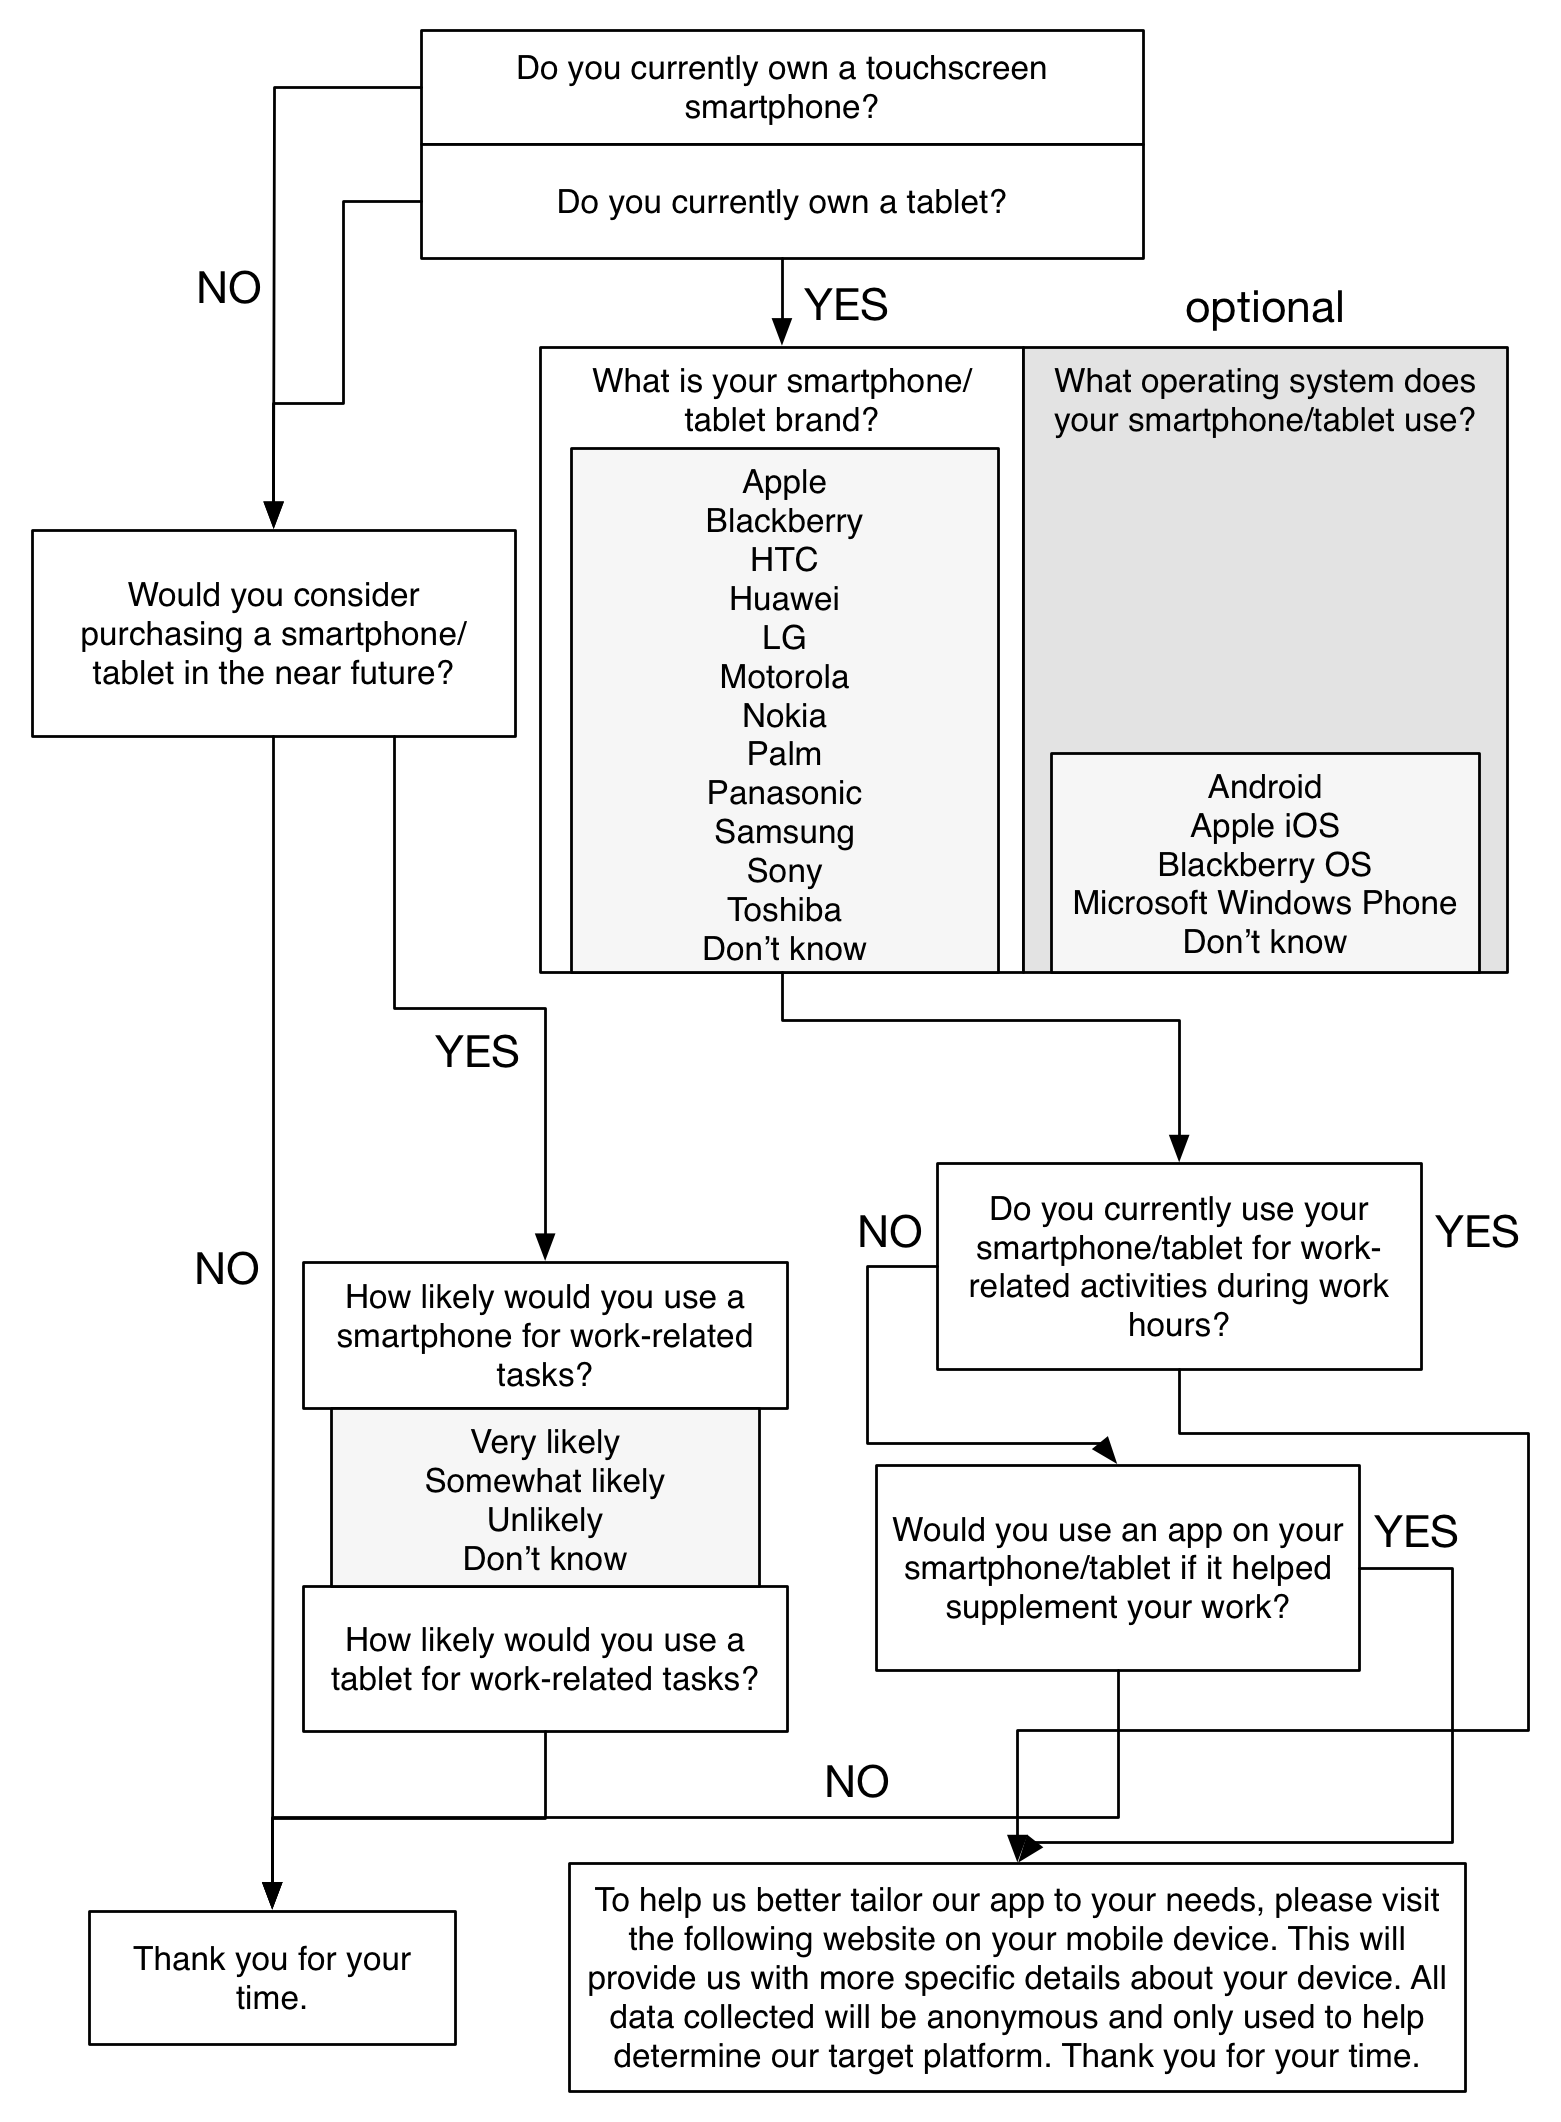
\includegraphics[scale=0.53]{img/device-survey.png}
\caption{Initial survey flow}
\end{figure}
\\
It was decided through client feedback that the survey flow logic could be replaced with a simple one-page linear survey due to the straightforward nature of the questions. The contents of the final survey are below.
\paragraph{Final SurveyMonkey Survey}
\begin{enumerate}
\item Do you currently own a touchscreen smartphone or a tablet?
\begin{enumerate}
\item Smartphone only
\item Tablet only
\item Smartphone and tablet
\item Neither
\end{enumerate}
\item Would you consider purchasing a smartphone/tablet in the near future?
\begin{enumerate}
\item Yes
\item No
\end{enumerate}
\item What is your smartphone/tablet brand?
\begin{enumerate}
\item Apple
\item Blackberry
\item HTC
\item Huawei
\item LG
\item Motorola
\item Nokia
\item Palm
\item Panasonic
\item Samsung
\item Sony
\item Toshiba
\item Other (please specify) \\
\framebox[8cm]{}
\end{enumerate}
\item What operating system does your smartphone/tablet use (if known)?
\begin{enumerate}
\item Android
\item Apple iOS
\item Blackberry OS
\item Microsoft Windows Phone
\item Other (please specify) \\
\framebox[8cm]{}
\end{enumerate}
\item Do you currently use your smartphone/tablet for work-related activities during work hours?
\begin{enumerate}
\item Yes
\item No
\end{enumerate}
\item Would you use an app on your smartphone/tablet if it helped supplement your work?
\begin{enumerate}
\item Yes
\item No
\end{enumerate}
\item How likely would you be to use a smartphone for work-related tasks?
\begin{enumerate}
\item Very likely
\item Somewhat likely
\item Unlikely
\item Don't know
\end{enumerate}
\item How likely would you be to use a tablet for work-related tasks?
\begin{enumerate}
\item Very likely
\item Somewhat likely
\item Unlikely
\item Don't know
\end{enumerate}
\item To help us better tailor our app to your needs, please visit the following website on your mobile device \url{http://goo.gl/KEevis}. This will provide us with more specific details about your device. All data collected will be anonymous and only used to help determine our target platform. Please feel free to add any comments.\\
\framebox[8cm]{}
\end{enumerate}  

\newpage
\section{Internal Meetings and Documentation}
\label{sec:internal_meetings}
\end{document}